%==============================================================================
%  Quantum machine learning for AIS maritime anomaly detection
%
%  Target: IEEE Transactions on Quantum Engineering (two-column journal).
%  For an IEEE conference (e.g. QCE) change the class option to [conference].
%
%  COMPILE
%    Overleaf: upload this folder, set main.tex as the main document.
%    Local:    latexmk -pdf main.tex   (needs MiKTeX or TeX Live)
%
%  RULES FOR THIS FILE
%    * Tables in tables/ are GENERATED by scripts/27_paper_tables.py. Never edit
%      them here; re-run the script if a number changes.
%    * Figures come from ../figures/ and are produced by scripts/24_figures.py.
%    * Every reference lives in refs.bib and was verified against Crossref or
%      OpenAlex. Do not add one from memory.
%    * Each section below starts with a WRITE block: what the section must do,
%      which numbers to quote, and the trap to avoid. Delete it as you write.
%      Full guidance: docs/PAPER_OUTLINE.md
%==============================================================================
\documentclass[journal]{IEEEtran}

\usepackage{graphicx}
\usepackage{booktabs}
\usepackage{amsmath}
\usepackage{amssymb}
\usepackage{url}
\usepackage{cite}
\usepackage[hidelinks,breaklinks]{hyperref}

\graphicspath{{../figures/}{figures/}}

\begin{document}

\title{Quantum Models Need More Data, Not Less: A Controlled Test of
Generalization-Bound Predictions in Maritime AIS Anomaly Detection}

\author{Jonathan Thomas% <- affiliation and contact go here
\thanks{Code, data and every result file: \url{https://github.com/AussAmerishFire/qml-ais-code}}}

\markboth{}{}
\maketitle

%------------------------------------------------------------------ abstract
\begin{abstract}
% WORKING DRAFT -- revise this last, once every other section is final.
% 219 words; IEEE journals allow up to 250. Every number is from
% docs/COMPLETE_RESULTS.md or results/final_results.csv.
The Automatic Identification System (AIS) underpins maritime surveillance, yet
vessels can falsify their reports or switch off their transponders. Labeled
examples of such behavior are scarce, and quantum machine learning is often
expected to help in exactly this regime: generalization bounds for quantum
models scale with the number of trainable gates, suggesting that small quantum
models should learn well from few examples. We test this expectation under
controlled conditions. From 8.2 million AIS reports we construct 114,969
ten-report windows described by twelve engineered features, and inject five
attack types into 3.47\% of them. We compare three 8-qubit hybrid quantum neural
networks against classical twins matched in depth and parameter count, a
quantum-kernel support vector machine, and six classical baselines, at five
training-set sizes from 571 to 68,296 windows, using vessel-disjoint splits and
1,222 model fits. Against their matched twins, the quantum networks are
significantly worse when training data are scarce and significantly better when
they are plentiful: no significant wins and six losses at 571 windows, nineteen
wins and no losses at 68,296, with crossovers between 2,443 and 9,432 windows.
No quantum model outperforms gradient boosting at any size (test AUC 0.832
versus 0.807). The quantum kernel does not degrade with scarce data, which
locates the deficit in variational optimization, and the geometric difference
between quantum and classical kernels reaches only about one tenth of its
theoretical maximum.
\end{abstract}

\begin{IEEEkeywords}
Quantum machine learning, anomaly detection, maritime surveillance, Automatic
Identification System, quantum kernels, variational quantum circuits,
generalization.
\end{IEEEkeywords}

%--------------------------------------------------------------- introduction
\section{Introduction}
\label{sec:intro}
% DRAFT -- rewrite in your own words before submission. ~830 words.

\IEEEPARstart{T}{he} Automatic Identification System (AIS) requires large
commercial vessels to broadcast their identity, position, speed and course at
intervals of seconds to minutes, and it has become the primary data source for
maritime surveillance. Because these broadcasts are self-reported, they can be
manipulated: a vessel can transmit false positions, misreport its speed, or
switch its transponder off entirely. Such behavior conceals sanctions evasion,
illegal fishing and unsafe operation. Satellite imagery shows that a large share
of industrial activity at sea is absent from public tracking
systems~\cite{paolo2024satellite}, and deliberate disabling of AIS concentrates
in identifiable hot spots~\cite{welch2022unseen}.

Detecting these anomalies automatically is an established
problem~\cite{riveiro2018review}. Approaches range from statistical models of
normal traffic~\cite{pallotta2013tread,millefiori2016ou} to deep networks
trained on raw trajectories~\cite{kroodsma2018fisheries,nguyen2021geotracknet}.
On engineered tabular features, tree ensembles such as gradient boosting remain
difficult to outperform~\cite{grinsztajn2022trees,shwartzziv2022tabular}. All of
these methods share one constraint: they learn from labeled examples, and
confirmed cases of spoofing or transponder switch-off are rare and costly to
verify.

Quantum machine learning has been proposed as a way to learn from such limited
data~\cite{biamonte2017qml,havlicek2019supervised}. Caro
\textit{et al.}~\cite{caro2022generalization} showed that the generalization
error of a quantum model with $T$ trainable gates, trained on $N$ examples, is
bounded by approximately $\sqrt{T/N}$. A natural reading of this result is that
small quantum models should generalize well from few examples, and therefore
that quantum machine learning should be most useful precisely when labels are
scarce. Maritime anomaly detection is a direct test of that reading: labels are
scarce, missed detections are costly, and the inputs are low-dimensional enough
to be encoded on a small number of qubits.

Whether quantum models deliver this advantage in practice is unclear. A
large-scale benchmark found that standard classical models systematically
outperformed the quantum classifiers it tested~\cite{bowles2024benchmarking},
and it has been argued that asking \emph{under what conditions} quantum models
behave differently is more informative than asking whether they are
better~\cite{schuld2022advantage}. Quantum approaches to anomaly detection have
been surveyed~\cite{corli2025anomaly} and applied to multivariate time series
and to aviation surveillance data~\cite{tscharke2025autoencoder,naaman2025adsb}.
We are not aware of a study that compares quantum models on vessel-tracking data
against classical controls matched in depth and parameter count, across a range
of training-set sizes.

This paper asks: \emph{under what conditions do quantum machine learning models
outperform classical models in detecting anomalous vessel behavior in AIS data?}
We address four sub-questions:
\begin{enumerate}[\IEEEsetlabelwidth{(SQ4)}]
  \item[(SQ1)] Against a classical model of equal depth and parameter count,
  does the comparison depend on training-set size?
  \item[(SQ2)] Do quantum models outperform the strongest classical models?
  \item[(SQ3)] Do quantum kernels behave differently from variational quantum
  circuits?
  \item[(SQ4)] Is there a measurable ceiling on quantum advantage for these data?
\end{enumerate}

Our contributions are as follows.
\begin{itemize}
  \item A controlled comparison of three 8-qubit hybrid quantum neural networks
  against classical twins matched in depth and parameter count, a quantum-kernel
  support vector machine, and six classical baselines, at five training-set
  sizes spanning a 120-fold range, using vessel-disjoint splits and 1,222 model
  fits.
  \item Evidence that the quantum--classical gap inverts with training-set size,
  in the direction opposite to the common reading of the bound: the quantum
  models are significantly worse with scarce data and significantly better with
  plentiful data, in two of three architectures.
  \item A frozen-circuit ablation showing that training the quantum gates makes
  no measurable difference at any training-set size, and a comparison with a
  quantum kernel that locates the scarce-data deficit in variational
  optimization rather than in quantum feature maps.
  \item A measured ceiling on quantum-kernel advantage for these data, using the
  geometric difference of Huang \textit{et al.}~\cite{huang2021power}, and a
  negative result for quantum features added to the tree ensembles used in
  practice.
  \item A public release of the data pipeline, code and every result file.
\end{itemize}

Section~\ref{sec:related} reviews related work. Section~\ref{sec:data}
describes the data and the injected attacks, and Section~\ref{sec:method} the
models and experimental design. Section~\ref{sec:results} reports the results
by sub-question, Section~\ref{sec:discussion} discusses them, and
Sections~\ref{sec:limitations} and~\ref{sec:future} set out limitations and
future work.

%-------------------------------------------------------------- related work
\section{Related Work}
\label{sec:related}
% DRAFT -- rewrite in your own words before submission.

\subsection{Maritime Anomaly Detection}
Riveiro \textit{et al.}~\cite{riveiro2018review} review maritime anomaly
detection and group existing methods into rule-based, statistical and
learning-based approaches. Statistical approaches model normal traffic and flag
departures from it: Pallotta \textit{et al.}~\cite{pallotta2013tread} extract
route patterns from historical AIS data by clustering, and Millefiori
\textit{et al.}~\cite{millefiori2016ou} model vessel motion as a mean-reverting
stochastic process for long-term prediction. Learning-based approaches operate
on raw trajectories. Kroodsma \textit{et al.}~\cite{kroodsma2018fisheries}
applied convolutional neural networks to AIS tracks to map fishing activity
worldwide; GeoTrackNet~\cite{nguyen2021geotracknet} detects anomalies with a
probabilistic recurrent representation of AIS tracks and an \textit{a contrario}
detector; and TrAISformer~\cite{nguyen2021traisformer} predicts trajectories
with a transformer. Paolo \textit{et al.}~\cite{paolo2024satellite} matched
satellite imagery against AIS and showed how much industrial activity escapes
AIS altogether. These methods differ in how they model normal behavior, but none
examines how detection degrades as labeled examples become scarce, which is the
regime in which quantum models are expected to help.

\subsection{Tree Ensembles as the Practical Baseline}
On tabular data, tree ensembles remain strong. Grinsztajn
\textit{et al.}~\cite{grinsztajn2022trees} found that tree-based models still
outperform deep learning on typical medium-sized tabular datasets, and
Shwartz-Ziv and Armon~\cite{shwartzziv2022tabular} found that gradient-boosted
trees generally outperformed recently proposed deep models for tabular data.
Because our features are engineered and tabular, gradient boosting and random
forest are the relevant comparison for any claim that a quantum model is useful
in practice.

\subsection{Quantum Machine Learning on Classical Data}
Two families of quantum models are commonly applied to classical
data~\cite{biamonte2017qml}. Variational quantum circuits encode the input as
gate parameters and train further gate angles by gradient
descent~\cite{cerezo2021vqa}; hybrid quantum neural networks combine such
circuits with classical layers. Quantum kernel methods instead use a fixed
circuit as a feature map and train a classical support vector machine on the
resulting kernel~\cite{havlicek2019supervised}. The way data are encoded
matters: repeating the encoding between trainable layers, known as data
re-uploading, makes even a single qubit a universal
classifier~\cite{perezsalinas2020reuploading} and enlarges the set of functions
a circuit can express~\cite{schuld2021encoding}. Huang
\textit{et al.}~\cite{huang2021power} showed that whether any quantum kernel
can outperform classical kernels on a given dataset can be bounded from the
data themselves, through a quantity they call the geometric difference. We
compute it in Section~\ref{sec:sq4}.

\subsection{Generalization Bounds and Benchmarking}
Caro \textit{et al.}~\cite{caro2022generalization} proved that the
generalization error of a quantum model with $T$ trainable gates trained on $N$
examples scales at worst as $\sqrt{T/N}$, improving to $\sqrt{K/N}$ when only
$K \ll T$ gates change substantially during training. These are upper bounds on
the gap between training and test performance; they do not guarantee that
training succeeds. Gil-Fuster \textit{et al.}~\cite{gilfuster2024rethinking}
showed that quantum models can fit randomly labeled data, so uniform bounds of
this kind cannot by themselves explain when quantum models generalize. On the
empirical side, Bowles \textit{et al.}~\cite{bowles2024benchmarking}
benchmarked a range of popular quantum classifiers and found that standard
classical models systematically outperformed them, and Schuld and
Killoran~\cite{schuld2022advantage} argued that the field should study when and
why quantum models behave differently rather than seek a blanket advantage.

\subsection{Quantum Anomaly Detection}
Corli \textit{et al.}~\cite{corli2025anomaly} review quantum machine-learning
algorithms for anomaly detection. Applications include a quantum autoencoder
for multivariate time series~\cite{tscharke2025autoencoder} and quantum-enhanced
anomaly detection on ADS-B data~\cite{naaman2025adsb}, the aviation counterpart
of AIS. To our knowledge, none of this work compares quantum models with
classical controls matched in depth and parameter count across a range of
training-set sizes, which is the comparison needed to test the scarce-data
argument directly.

%------------------------------------------------------------------ the data
\section{Data and Problem Setup}
\label{sec:data}
% DRAFT -- rewrite in your own words before submission.
Fig.~\ref{fig:overview} summarizes the data pipeline and the experiment.

\begin{figure*}[t]
  \centering
  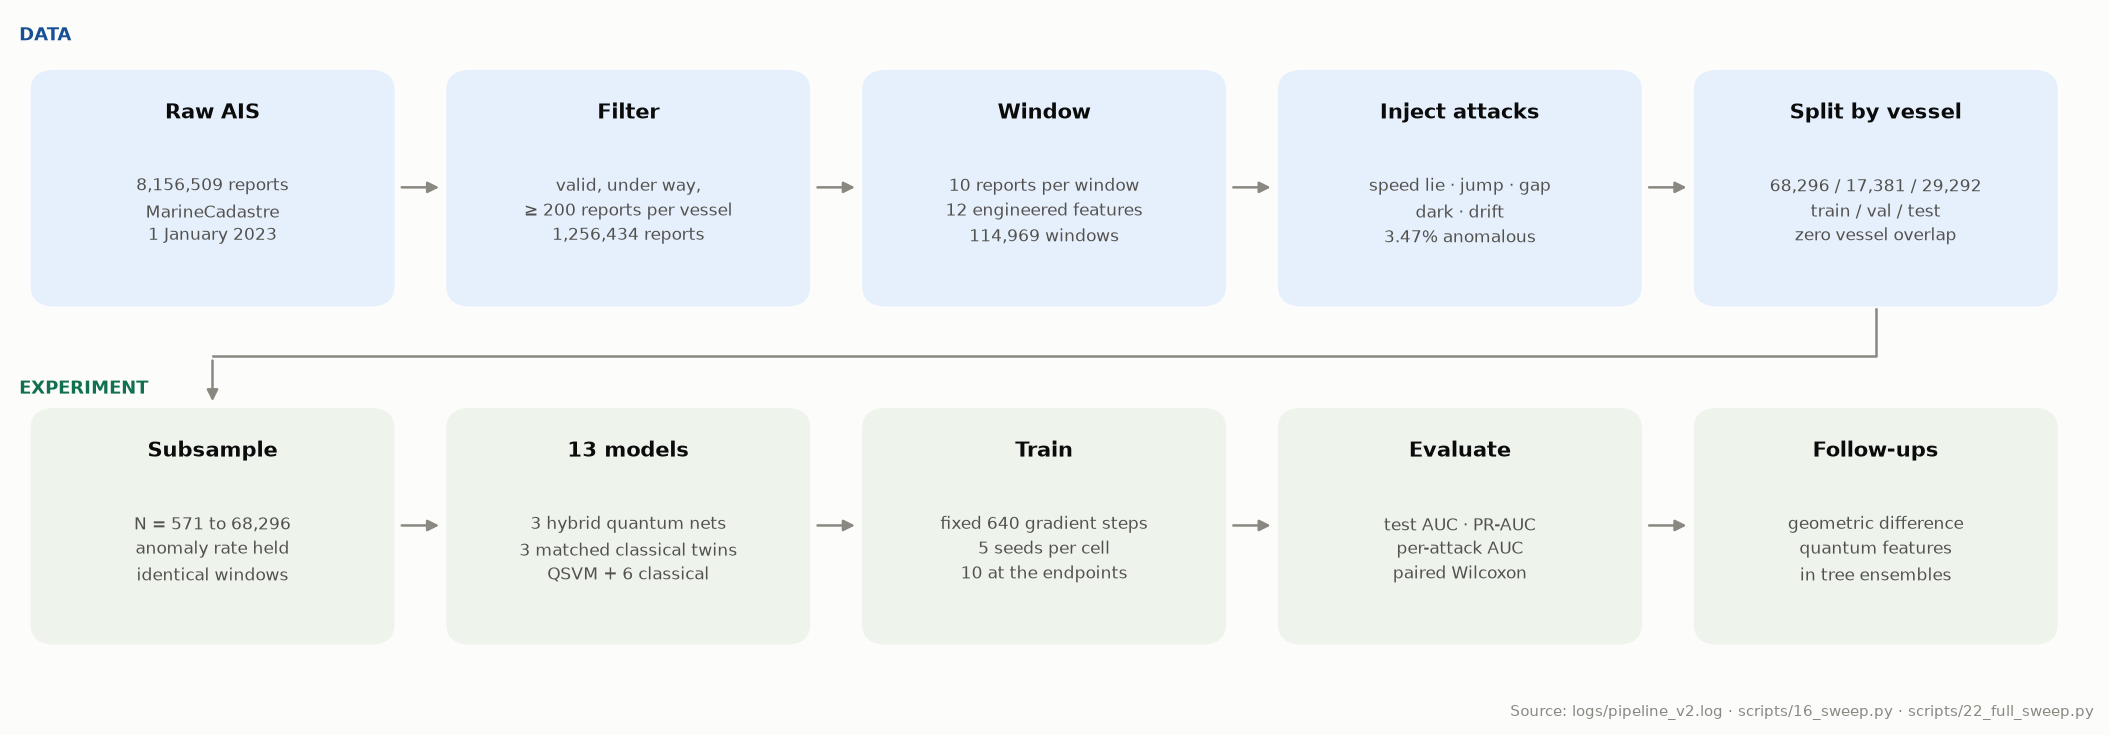
\includegraphics[width=\textwidth]{15_method_overview.png}
  \caption{The study as one flow, with the real count at every stage. The data
  pipeline (top) feeds the experiment (bottom).}
  \label{fig:overview}
\end{figure*}

\subsection{Source Data and Windowing}
We obtained every AIS position report broadcast off the coast of the United
States on 1 January 2023 from MarineCadastre~\cite{marinecadastre}: 8,156,509
reports from 15,932 vessels. We retained reports from Class A transceivers, the
system mandatory for large commercial vessels; excluded speeds of 40~kn or more,
which removes the value 102.3 that AIS uses to encode an unavailable speed; and
excluded speeds below 0.5~kn, which removes moored vessels and accounts for 76\%
of the remaining reports. We then kept vessels with at least 200 reports,
leaving 1,256,434 reports from 2,441 vessels (Fig.~\ref{fig:pipeline}).

Each vessel's reports were sorted in time and segmented into voyages wherever
consecutive reports were more than 1,800~s apart, an interval that no normal
Class~A reporting interval in the data reaches. This produced 7,935 voyages.
Segmentation preceded every calculation between consecutive reports, so that no
quantity was computed across two voyages. Each voyage was then partitioned into
non-overlapping windows of ten consecutive reports, which span about
12~minutes at the median reporting interval of 70~s. The windows do not overlap
so that no two windows share a report.

\subsection{Features}
For each pair of consecutive reports we computed the elapsed time, the
great-circle distance between the two positions, the speed implied by that
distance, the absolute difference between implied and reported speed (the
\emph{speed mismatch}), and the bearing actually travelled. From these we
derived twelve features per window, defined in Appendix~\ref{app:features}.
Most target internal contradictions rather than departures from typical
behavior: a vessel reports both its position and its speed, and the two must
agree. In unmodified data the median speed mismatch is 0.11~kn and its
99th percentile 3.20~kn.

Seven features summarize each window by a mean or a maximum. Because a maximum
cannot capture a gradual trend, we added four trend and direction features (the
angle between reported course and the bearing travelled, the slope of the speed
mismatch across the window, the straightness of the path, and the mean speed
mismatch) together with a flag for missing heading. On a held-out
vessel-disjoint split, adding the four features raised random-forest AUC from
0.790 to 0.833. Seven heavy-tailed features were log-transformed, the mismatch
slope was given a signed logarithm, and every feature was min--max scaled to
$[0,\pi]$ using training-split statistics only, because each value is later
encoded as a qubit rotation angle. Fig.~\ref{fig:features} shows how well each
feature separates each attack on its own.

\subsection{Injected Attacks}
No public dataset labels AIS manipulation at this scale, so we injected five
attack types with known labels (Fig.~\ref{fig:attackex}). \emph{Speed
falsification} multiplies or divides the reported speed from a random point
onward by a factor of 1.8--5.0, limited so that the reported speed stays between
0.5 and 39~kn. A \emph{position jump} displaces every later position by
500--20,000~m on a random bearing. A \emph{reporting gap} deletes consecutive
reports until 500--1,700~s of silence accumulate; the lower bound exceeds the
99th percentile of natural gaps (491~s), and the upper bound stays below the
1,800~s voyage threshold so that the gap does not split the voyage.
\emph{Transponder switch-off} deletes 3,600--21,600~s of reports, splitting the
voyage so that its second part begins after a long silence. \emph{Gradual drift}
displaces positions along a random bearing by up to 100--3,000~m, growing as
$(i/n)^{1.5}$ along the track, while leaving speed, course and heading
unchanged. Severities were drawn uniformly from these ranges
(Appendix~\ref{app:attacks}).

Of 5,900 eligible voyages, 2,653 (45\%) were attacked. Because attacks corrupt
very different numbers of reports (speed falsification affects hundreds; a
position jump, three), voyages were allocated to attacks in inverse proportion
to the windows each produces, which reduced the imbalance between attack types
from 128:1 to 2.3:1. A window was labeled anomalous only if it contained at least
one modified report. Finally, 77 normal windows whose speed mismatch exceeded
60~kn were removed as corrupted position data. The resulting dataset contains
114,969 windows, of which 3,992 (3.47\%) are anomalous. Gradual drift is the
largest class, at 37.7\% of test anomalies (Fig.~\ref{fig:attacks}).

\subsection{Vessel-Disjoint Splitting}
Windows were partitioned by vessel into training (60\%), validation (15\%) and
test (25\%) sets, so that every window from a given vessel falls in one split
and every model is evaluated on vessels it has never seen. Before assignment,
vessels were stratified by their dominant attack type and number of anomalous
windows, which keeps the attack mix comparable across splits.
Table~\ref{tab:dataset} gives the resulting splits; no vessel appears in more
than one. Splitting by window instead would place windows from the same voyage
on both sides of the split and inflate every score.

\subsection{Class Imbalance and the Alert Budget}
With 3.47\% of windows anomalous, a detector that flags nothing achieves 96.5\%
accuracy, so we do not report accuracy. We report the area under the receiver
operating characteristic curve (AUC), which measures how reliably anomalous
windows are ranked above normal ones; the area under the precision--recall
curve (PR-AUC), which emphasizes the top of the ranking that an analyst would
review; and precision and recall when the highest-scoring 3.5\% of test windows
are flagged, a budget matching the anomaly rate.

% GENERATED by scripts/27_paper_tables.py -- do not edit by hand
\begin{table}[t]
\centering
\caption{The dataset. Splits are vessel-disjoint: no MMSI appears in more than one split.}
\label{tab:dataset}
\begin{tabular}{lrrrr}
\toprule
Split & Windows & Vessels & Anomalous & Rate \\
\midrule
Train & 68,296 & 1,462 & 2,420 & 3.54\% \\
Validation & 17,381 & 364 & 537 & 3.09\% \\
Test & 29,292 & 609 & 1,035 & 3.53\% \\
\bottomrule
\end{tabular}
\end{table}


\begin{figure}[t]
  \centering
  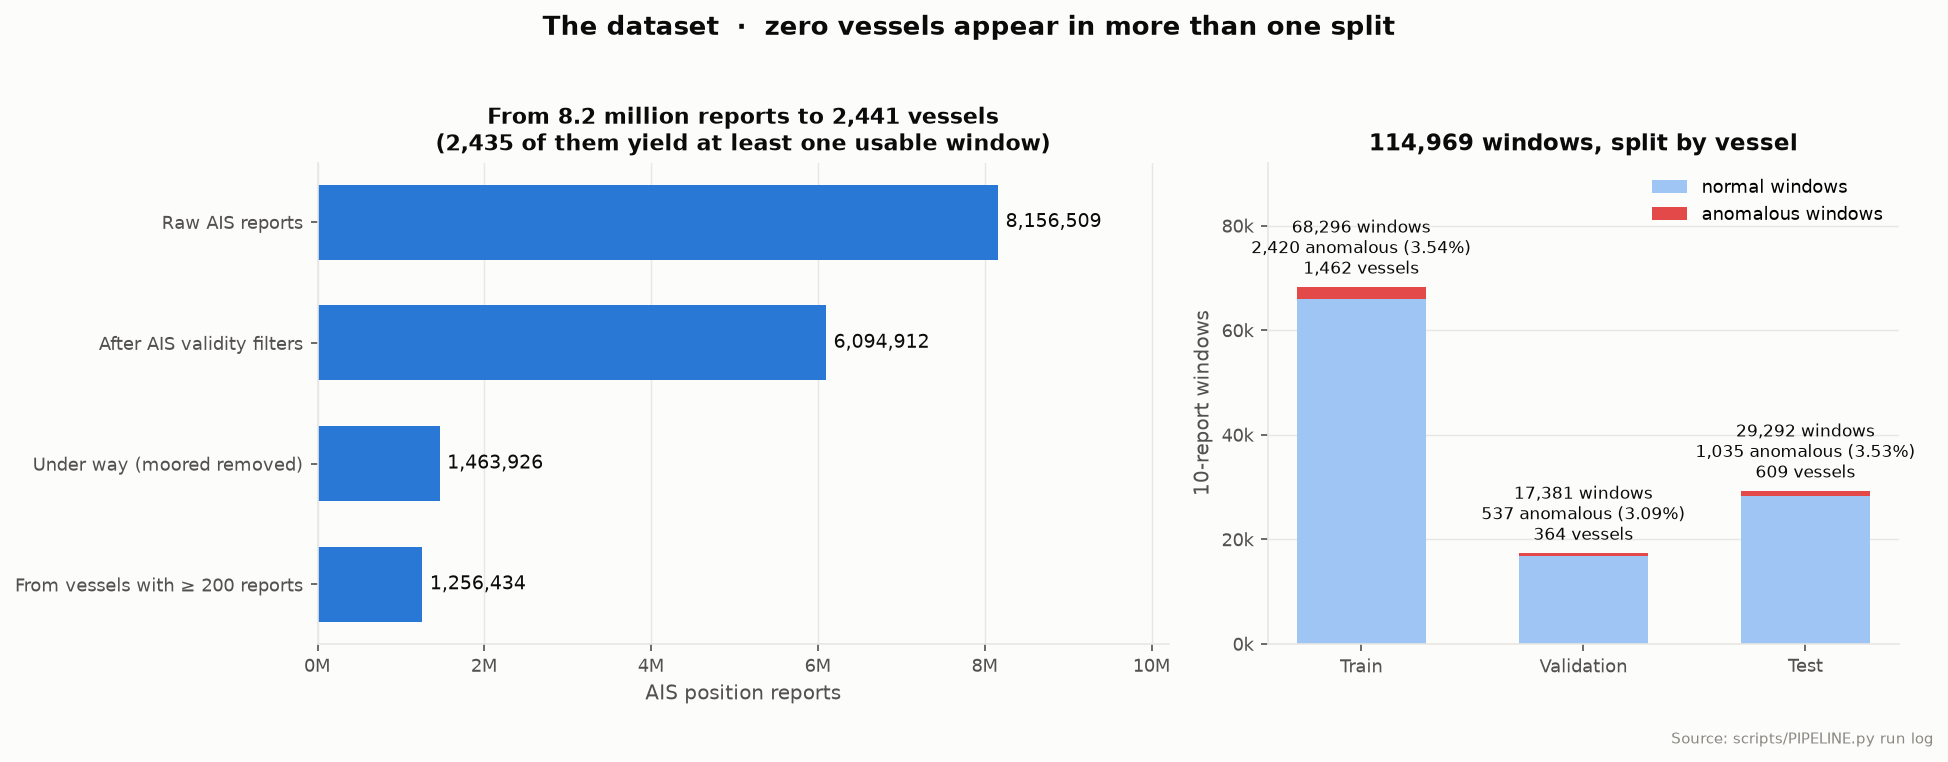
\includegraphics[width=\columnwidth]{01_data_pipeline.png}
  \caption{From 8.2 million raw AIS reports to 114,969 ten-report windows, and
  the vessel-disjoint split. No vessel appears in more than one split.}
  \label{fig:pipeline}
\end{figure}

\begin{figure*}[t]
  \centering
  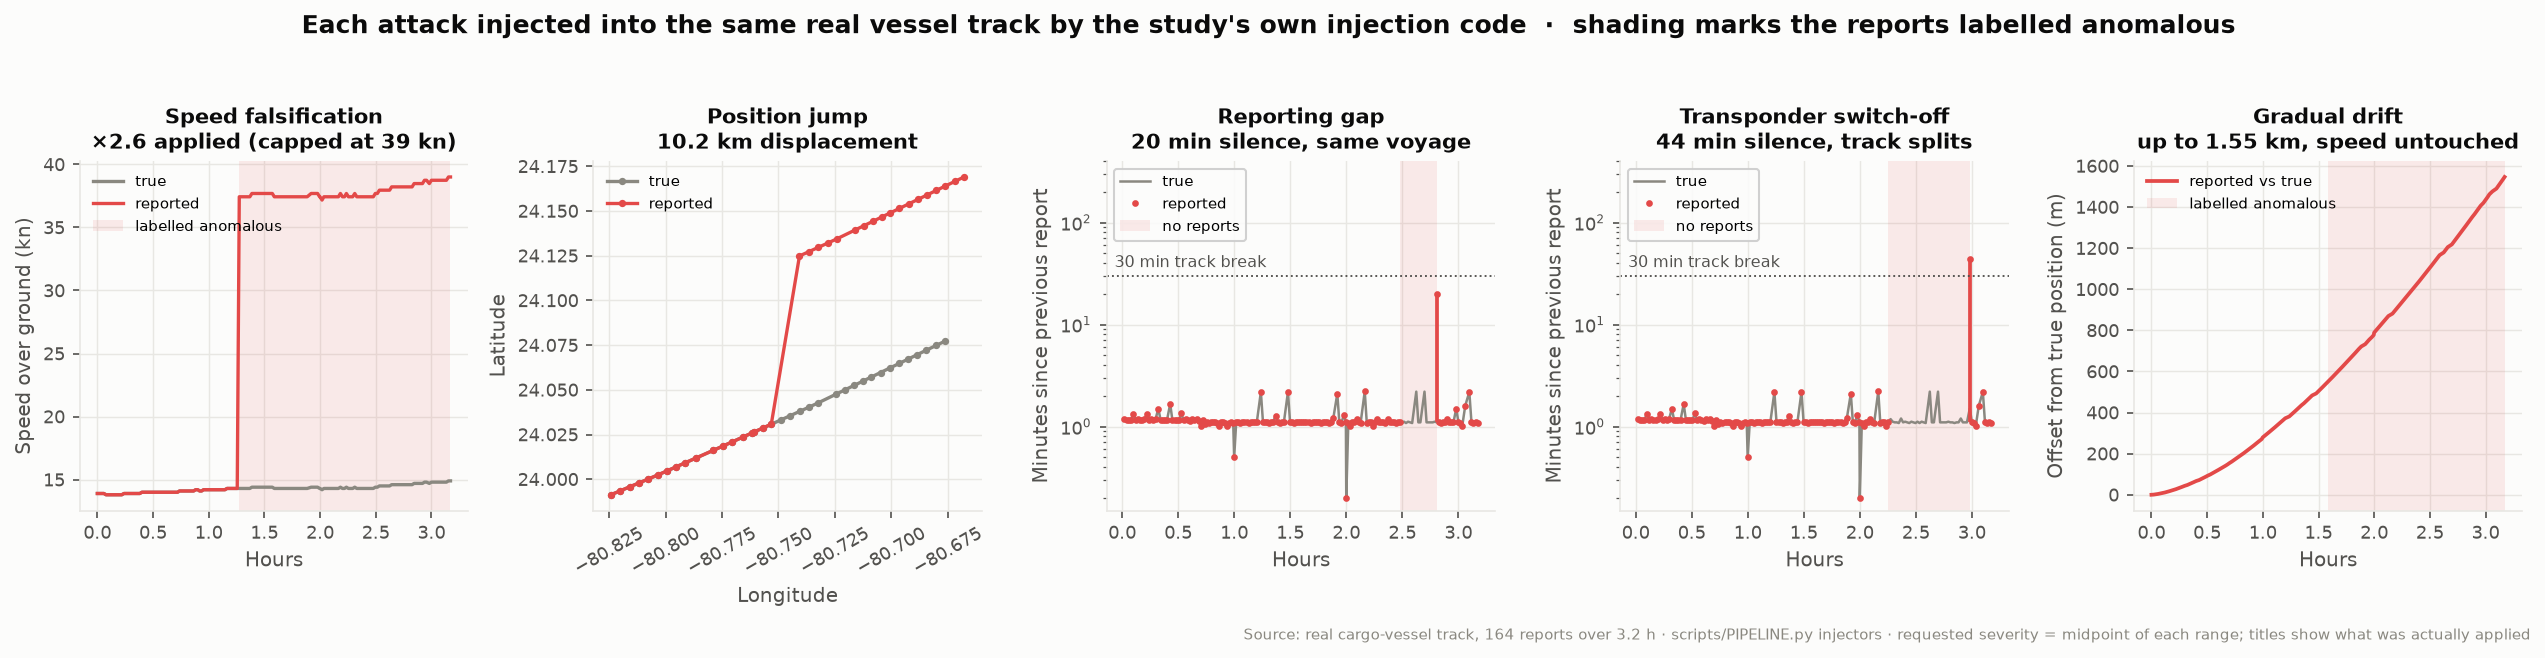
\includegraphics[width=\textwidth]{17_attack_examples.png}
  \caption{Each attack injected into the same real vessel track by the study's
  injection code. Shading marks the reports labeled anomalous. Panel titles give
  the severity actually applied, which can fall below the requested value where
  a physical limit binds (reported speed is capped at 39~kn).}
  \label{fig:attackex}
\end{figure*}

\begin{figure}[t]
  \centering
  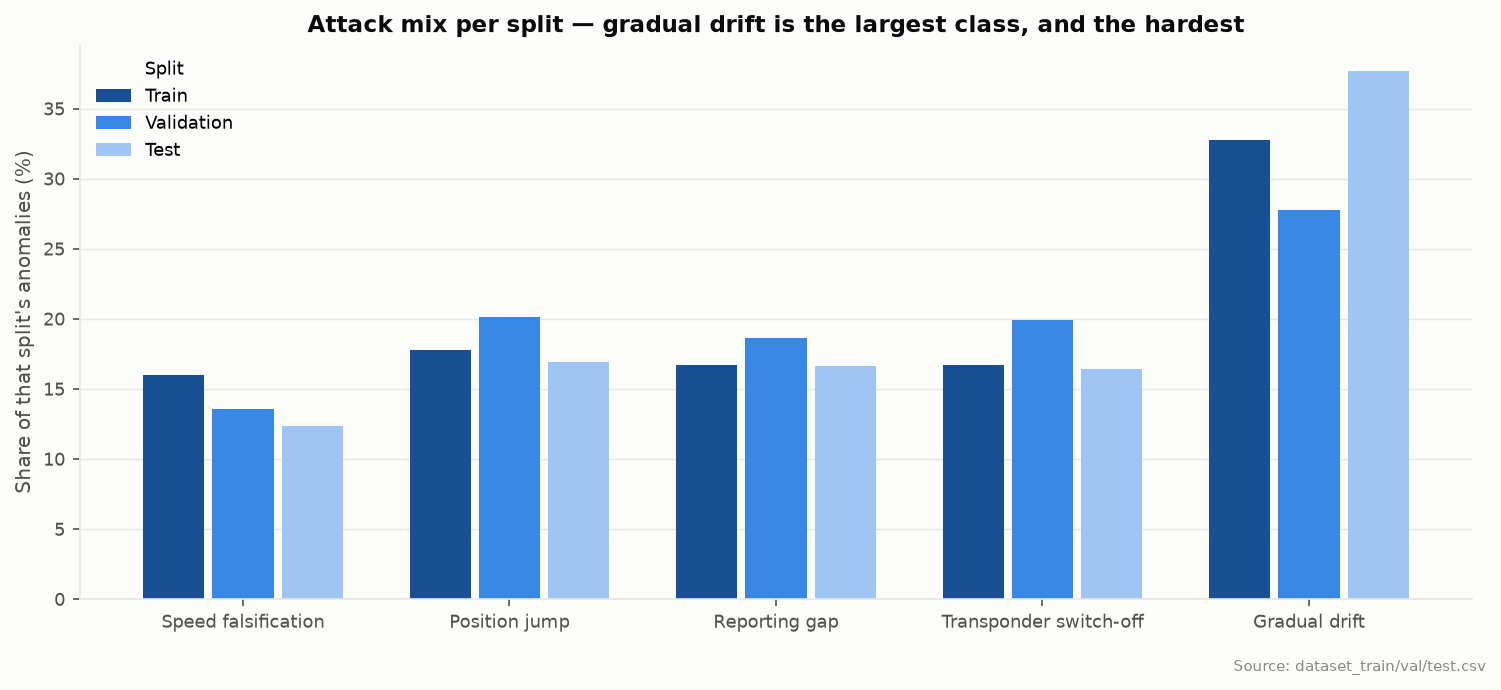
\includegraphics[width=\columnwidth]{02_attack_composition.png}
  \caption{Share of each attack type within each split's anomalies. Gradual
  drift is the largest class and, as Section~\ref{sec:results} shows, the
  hardest to detect.}
  \label{fig:attacks}
\end{figure}

\begin{figure}[t]
  \centering
  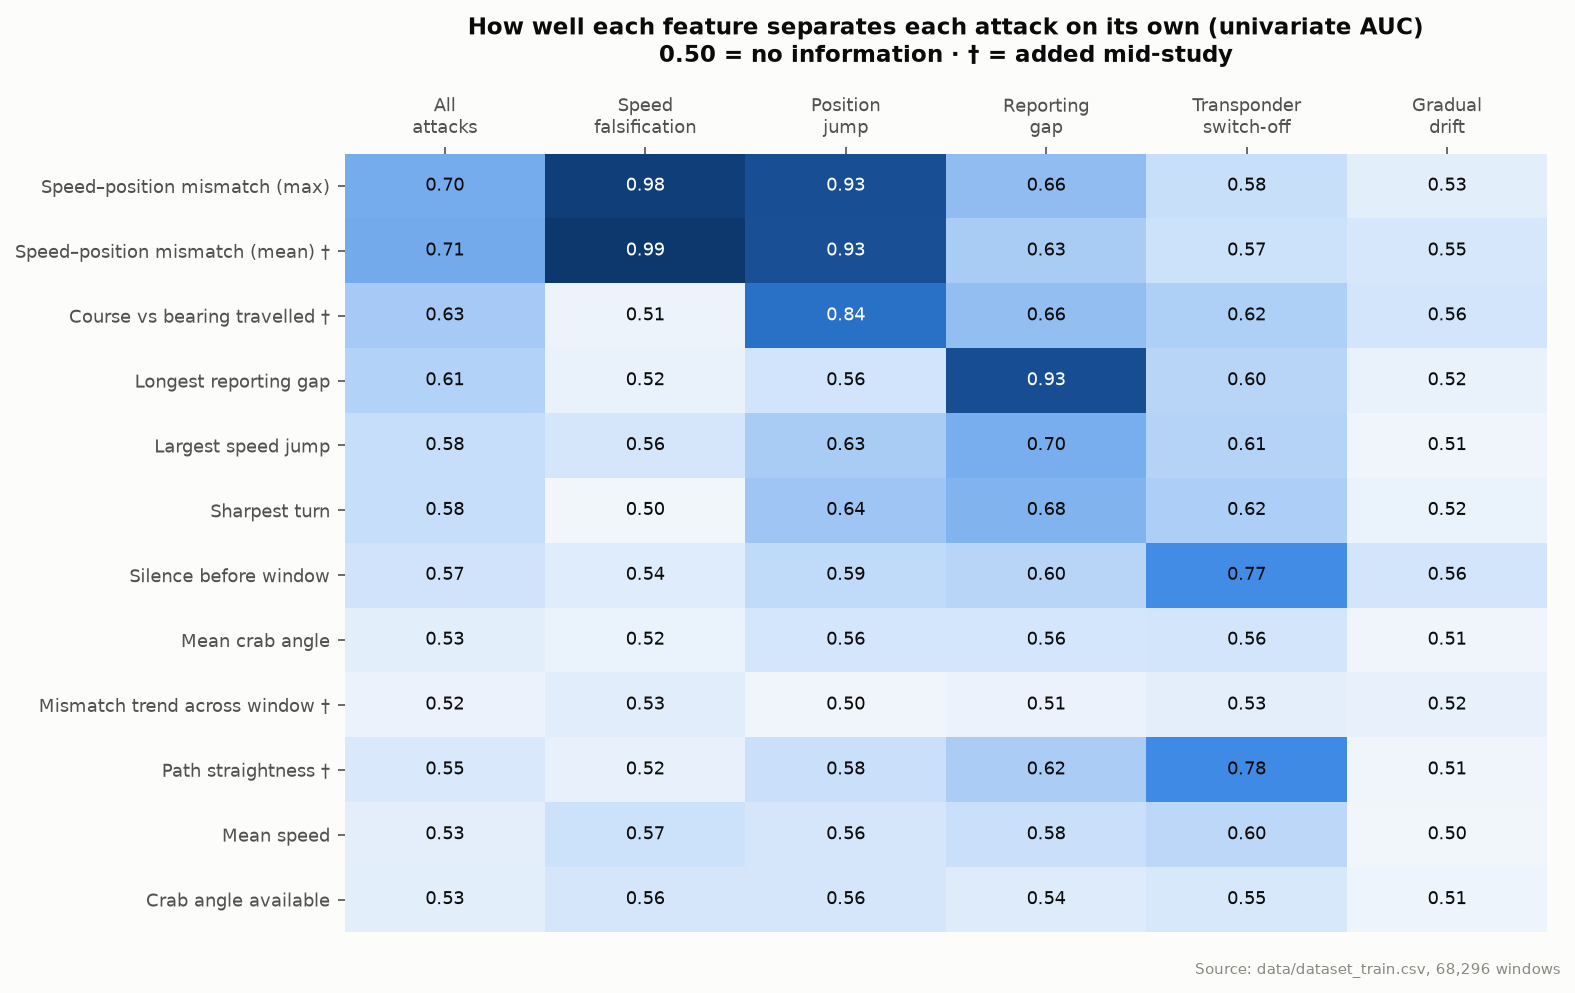
\includegraphics[width=\columnwidth]{03_feature_separability.png}
  \caption{Univariate AUC of each feature against each attack type. A value of
  0.50 means the feature carries no information about that attack on its own.}
  \label{fig:features}
\end{figure}

%----------------------------------------------------------------- the models
\section{Models and Experimental Design}
\label{sec:method}
% DRAFT -- rewrite in your own words before submission.
We compare thirteen models, listed with their parameter counts in
Table~\ref{tab:models}.

\subsection{Hybrid Quantum Neural Networks}
All three hybrid quantum neural networks (HQNNs) use eight qubits and share the
structure shown in Fig.~\ref{fig:circuits}. A trainable classical layer maps
the twelve features to eight rotation angles, $\boldsymbol{\theta} = \pi\,
\sigma(W\mathbf{x} + \mathbf{b})$, with $12\times 8$ weights and 8 biases
(104 parameters). This compression is forced by the qubit budget: angle
encoding places one feature on one qubit, and simulating twelve qubits costs
about sixteen times more per circuit evaluation than eight. It handicaps the
quantum models, whose classical twins read all twelve features directly. Each
angle is encoded as an $R_X$ rotation on its own qubit. Strongly entangling
layers then apply a general single-qubit rotation with three trainable angles
to every qubit, followed by a ring of CNOT gates; two layers contribute
$2\times 8\times 3 = 48$ trainable angles. The expectation value
$\langle Z_i\rangle$ is measured on each qubit, and a readout maps the eight
values to a single score, which a sigmoid converts to a probability. Circuits
were simulated exactly, without noise, using
PennyLane~\cite{bergholm2018pennylane}.

\begin{figure*}[t]
  \centering
  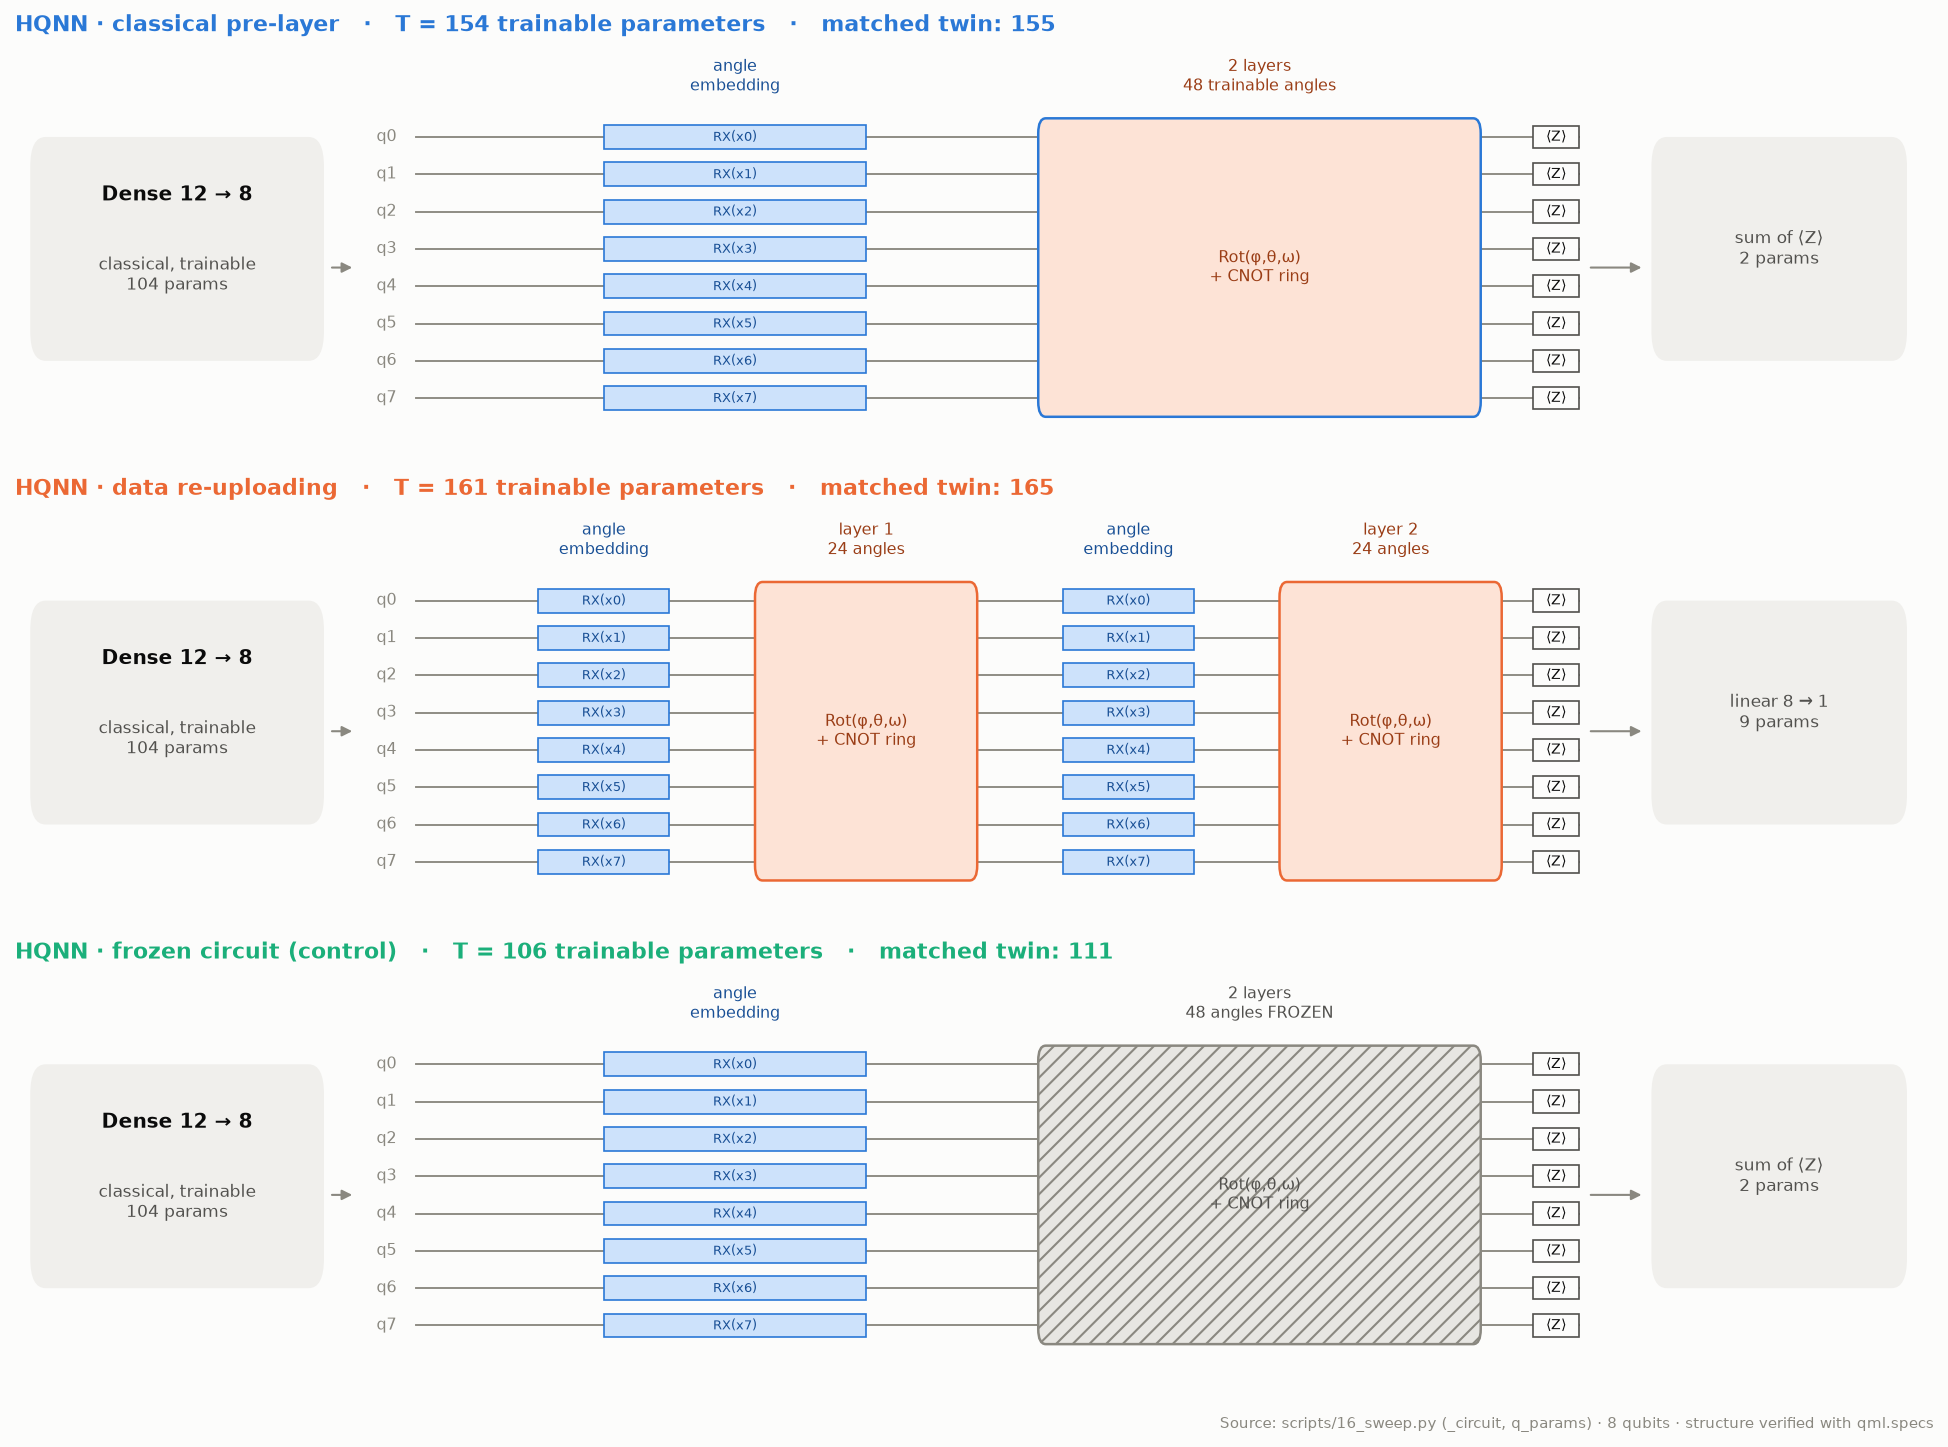
\includegraphics[width=\textwidth]{16_circuits.png}
  \caption{The three hybrid quantum architectures. Each compresses the 12
  features to 8 with a trainable classical layer, encodes them as qubit
  rotations, applies strongly entangling layers, and reads out Pauli-$Z$
  expectations. The frozen circuit is identical to the classical pre-layer
  model except that its 48 rotation angles are fixed at initialization.}
  \label{fig:circuits}
\end{figure*}

\subsubsection{Classical pre-layer}
The input is encoded once, followed by both entangling layers, with readout
$a\sum_i \langle Z_i\rangle + b$. The model has $T = 104 + 48 + 2 = 154$
trainable parameters.

\subsubsection{Data re-uploading}
The input is re-encoded before each entangling
layer~\cite{perezsalinas2020reuploading}, which enlarges the set of functions
the circuit can express~\cite{schuld2021encoding}, and the readout is a linear
combination of the eight expectation values (9 parameters), giving $T = 161$.

\subsubsection{Frozen-circuit control}
This model is identical to the pre-layer model, except that its 48 rotation
angles are fixed at their random initial values and never trained, giving
$T = 106$. Comparing it with the pre-layer model isolates what training the
quantum gates contributes.

\subsection{Depth- and Parameter-Matched Classical Twins}
Each HQNN is paired with a classical multilayer perceptron (MLP) of equal depth
and at least as many parameters. Because each HQNN has two trainable stages, its
twin has two hidden layers: 8 and 5 units for the pre-layer model
(155 parameters), 8 and 6 for the re-uploading model (165), and 6 and 4 for the
frozen circuit (111). Matching depth as well as parameter count matters: in a
preliminary two-seed screen, matching parameters alone produced an apparent
quantum advantage that disappeared once depth was also matched. The twins
receive all twelve features, the same training windows, and the same number of
optimization steps as their quantum counterparts.

\subsection{The Quantum Kernel}
The quantum support vector machine (QSVM) has no trainable circuit parameters.
The twelve features are reduced to eight by principal component analysis fitted
on the training subsample, rescaled to $[0,\pi]$, and mapped to quantum states
with an IQP embedding~\cite{havlicek2019supervised}. The kernel between two
windows is the fidelity $|\langle\phi(\mathbf{x})|\phi(\mathbf{x}')\rangle|^2$,
obtained by applying the embedding of $\mathbf{x}$ followed by the inverse
embedding of $\mathbf{x}'$ and reading the probability of the all-zero state. A
classical support vector machine is trained on the precomputed kernel, with its
regularization constant $C\in\{1, 10\}$ selected on a 20\% holdout drawn from
the training subsample. The kernel requires one circuit evaluation per pair of
windows, so its cost grows as $N^2$: about one hour per seed at 571 windows and
2.8~h at 1,429 on our hardware. At 68,296 windows the kernel matrix alone would
occupy 37~GB. We therefore evaluated the QSVM at the two smallest training-set
sizes, on the validation set.

\subsection{Classical Baselines}
We include six classical baselines (Table~\ref{tab:models}): gradient boosting,
random forest, logistic regression, an MLP with one hidden layer of five units
(71 parameters), an isolation forest trained without labels, and a
single-threshold rule that scores each window by its maximum speed mismatch and
is not trained at all. The last two show what can be achieved without labels.
Each baseline was tuned over 9--12 configurations by validation AUC on the full
training set (Appendix~\ref{app:repro}), and the selected configuration was used
at every training-set size. The quantum models and their twins were tuned over
two configurations each (Section~\ref{sec:training}). This asymmetry favors the
classical baselines.

\subsection{Training Protocol}
\label{sec:training}
\textit{Training-set sizes.} We trained on $N$ = 571, 1,429, 2,857, 14,286 and
68,296 windows. The first four correspond to 20, 50, 100 and 500 labeled
anomalies at a 3.5\% anomaly rate ($N$ = anomalies$/0.035$); the last is the
full training split, with 2,420 anomalies. The sizes span a 120-fold range. For
each seed $s$, a subsample of size $N$ was drawn at a fixed anomaly rate with a
random generator seeded by $1000+s$, so that every model trained on identical
windows at a given size and seed.

\textit{Hyperparameters.} Each neural model was tuned on one 14,286-window
subsample over two learning rates and three seeds: Adam learning rates of 0.02
and 0.05 for the HQNNs, and 0.003 and 0.01 for the twins, each with weight
decay $10^{-4}$. The setting with the higher mean validation AUC was kept. The
frozen circuit inherited the setting chosen for the pre-layer model.

\textit{Fixed step budget.} Every neural model, quantum or classical, was
trained for exactly 640 gradient steps at every training-set size, with batch
size $\min(4096, N)$, binary cross-entropy loss, L2 weight decay of $10^{-4}$
and the Adam optimizer. Training for a fixed number of epochs instead would give
a model trained on 571 windows about 120 times fewer parameter updates than one
trained on 68,296, so that scarce data would be confounded with
under-training. The budget equals 40 epochs at full data (16 batches per epoch).
The model after the final step was evaluated, without early stopping.

\subsection{Evaluation and Statistics}
Hyperparameters were selected on the validation set; the test set
(29,292 windows from 609 vessels) was used only to report results. We report
AUC, PR-AUC, precision and recall at the 3.5\% alert budget (the 1,025
highest-scoring test windows), and per-attack AUC, computed on the normal
windows together with the windows of a single attack type.

Each model was trained with five seeds at every size, and with ten seeds at the
smallest and largest sizes, which we call the endpoints. A quantum model and its
twin train on identical windows, so their comparison is paired by seed, and we
test it with a two-sided Wilcoxon signed-rank test. With $n$ pairs, the
smallest attainable $p$-value is $2/2^n$: 0.0625 for five seeds, so significance
at $p<0.05$ is impossible, and 0.002 for ten. We therefore test significance at
the endpoints with ten seeds and report effect sizes across all five sizes.
Where the quantum--twin difference $\Delta$ changes sign between adjacent sizes
$N_i$ and $N_{i+1}$, we locate the crossover by linear interpolation in
$\log N$:
\begin{equation}
N^{*} = \exp\!\left[\ln N_i + t\,(\ln N_{i+1}-\ln N_i)\right],\quad
t = \frac{-\Delta_i}{\Delta_{i+1}-\Delta_i}.
\label{eq:crossover}
\end{equation}

\subsection{Validation and Reproducibility}
The dataset passed 42 automated property checks and a recomputation of its
features through an independent implementation (22 checks). Nine complete
rebuilds of the pipeline tested three preprocessing thresholds
(Appendix~\ref{app:repro}). Sixty runs repeated through a second script
reproduced the original results exactly. All experiments ran on a single
laptop with 22 CPU threads and 17~GB of memory, in about 66~h of computation.
The code, data pipeline and every result file are publicly available.

% GENERATED by scripts/27_paper_tables.py -- do not edit by hand
\begin{table}[t]
\centering
\caption{Model inventory. $T$ counts trainable parameters. Every hybrid quantum network is matched to a classical twin of equal depth whose parameter count is never lower.}
\label{tab:models}
\begin{tabular}{lrrl}
\toprule
Model & $T$ & Twin $T$ & Constraint \\
\midrule
HQNN, data re-uploading & 161 & 165 & matched twin \\
HQNN, classical pre-layer & 154 & 155 & matched twin \\
HQNN, frozen circuit (control) & 106 & 111 & matched twin \\
Twin of re-uploading HQNN & 165 & --- & matched to data re-uploading \\
Twin of pre-layer HQNN & 155 & --- & matched to classical pre-layer \\
Twin of frozen HQNN & 111 & --- & matched to frozen circuit (control) \\
Quantum SVM & 0 (kernel) & --- & none \\
Gradient boosting & --- & --- & none \\
Random forest & --- & --- & none \\
Logistic regression & 13 & --- & none \\
MLP (12-5-1) & 71 & --- & none \\
Isolation forest & --- & --- & no labels \\
Threshold rule & 0 & --- & no labels \\
\bottomrule
\end{tabular}
\end{table}


%---------------------------------------------------------------- the results
\section{Results}
\label{sec:results}
% DRAFT -- rewrite in your own words before submission.
Table~\ref{tab:testauc} reports test AUC for every model at every training-set
size. We present the results by sub-question.

\subsection{The Gap Inverts With Training-Set Size}
\label{sec:sq1}
Against their matched twins, the hybrid quantum networks are significantly
worse when training data are scarce and significantly better when they are
plentiful.

\subsubsection{Quantum against matched twins}
Table~\ref{tab:endpoints} gives the paired differences at the endpoints. With
571 training windows, the pre-layer and frozen-circuit networks trail their
twins by 0.058 ($p=0.027$) and 0.081 ($p=0.020$). With 68,296 windows, both
lead, by 0.020 ($p=0.010$) and 0.040 ($p=0.002$). Fig.~\ref{fig:seeds} shows
every seed: at full data the frozen circuit outperforms its twin on all ten
seeds, and the pre-layer network on nine. Across all 54 paired comparisons
(three pairs, two sizes and nine metrics), all 19 significant quantum wins occur
at full data and all 6 significant losses at 571 windows
(Fig.~\ref{fig:significance}).

\subsubsection{The crossover point}
Fig.~\ref{fig:inversion} traces the difference across all five sizes on the
test set. By (\ref{eq:crossover}), the frozen circuit overtakes its twin at
about 2,443 windows, or 87 labeled anomalies, and the pre-layer network at about
7,229 windows, or 256 labeled anomalies. These values are interpolated between
measured sizes, not extrapolated beyond them.

\subsubsection{Frozen-circuit ablation}
Freezing the 48 quantum angles made no measurable difference at any size. The
validation difference between the frozen and trained pre-layer networks ranged
from $-0.019$ to $+0.004$ across the five sizes, with no value significant
($p\ge 0.625$); on the test set with ten seeds it was $+0.004$ at 571 windows
($p=1.000$) and $-0.001$ at 68,296 ($p=0.922$). The model with fewer trainable
gates therefore showed none of the small-data benefit that the $\sqrt{T/N}$
reading predicts, and the full-data advantage over the twins does not depend on
training the quantum gates.

\subsubsection{The data re-uploading exception}
The re-uploading network differs significantly from its twin at neither
endpoint ($+0.016$, $p=0.557$ at 571 windows; $+0.009$, $p=0.160$ at 68,296)
and stays within 0.035 of it at every size. It was also the strongest quantum
network at 571 windows (test AUC 0.653). Re-encoding the input enlarges the set
of functions a circuit can express~\cite{schuld2021encoding}; our data suggest
it may also make training from few examples easier, but this experiment does not
establish why.

These results do not contradict the bound of Caro
\textit{et al.}~\cite{caro2022generalization}, which limits the gap between
training and test error and says nothing about how well a model can be trained
from $N$ examples. They contradict the inference drawn from it: that a quantum
model with fewer trainable gates should outperform a classical model of the same
size when data are scarce.

% GENERATED by scripts/27_paper_tables.py -- do not edit by hand
\begin{table}[t]
\centering
\caption{Quantum minus its matched classical twin on the test set, at the two endpoints. Ten paired seeds, Wilcoxon signed-rank.}
\label{tab:endpoints}
\begin{tabular}{lrrrr}
\toprule
Pair & $\Delta$ $N{=}571$ & $p$ & $\Delta$ $N{=}68{,}296$ & $p$ \\
\midrule
classical pre-layer & $-0.0582$$^{*}$ & 0.027 & $+0.0198$$^{*}$ & 0.010 \\
data re-uploading & $+0.0164$ & 0.557 & $+0.0087$ & 0.160 \\
frozen circuit (control) & $-0.0813$$^{*}$ & 0.020 & $+0.0395$$^{*}$ & 0.002 \\
\bottomrule
\end{tabular}
\\[2pt]\footnotesize $^{*}$ $p<0.05$.
\end{table}


\begin{figure}[t]
  \centering
  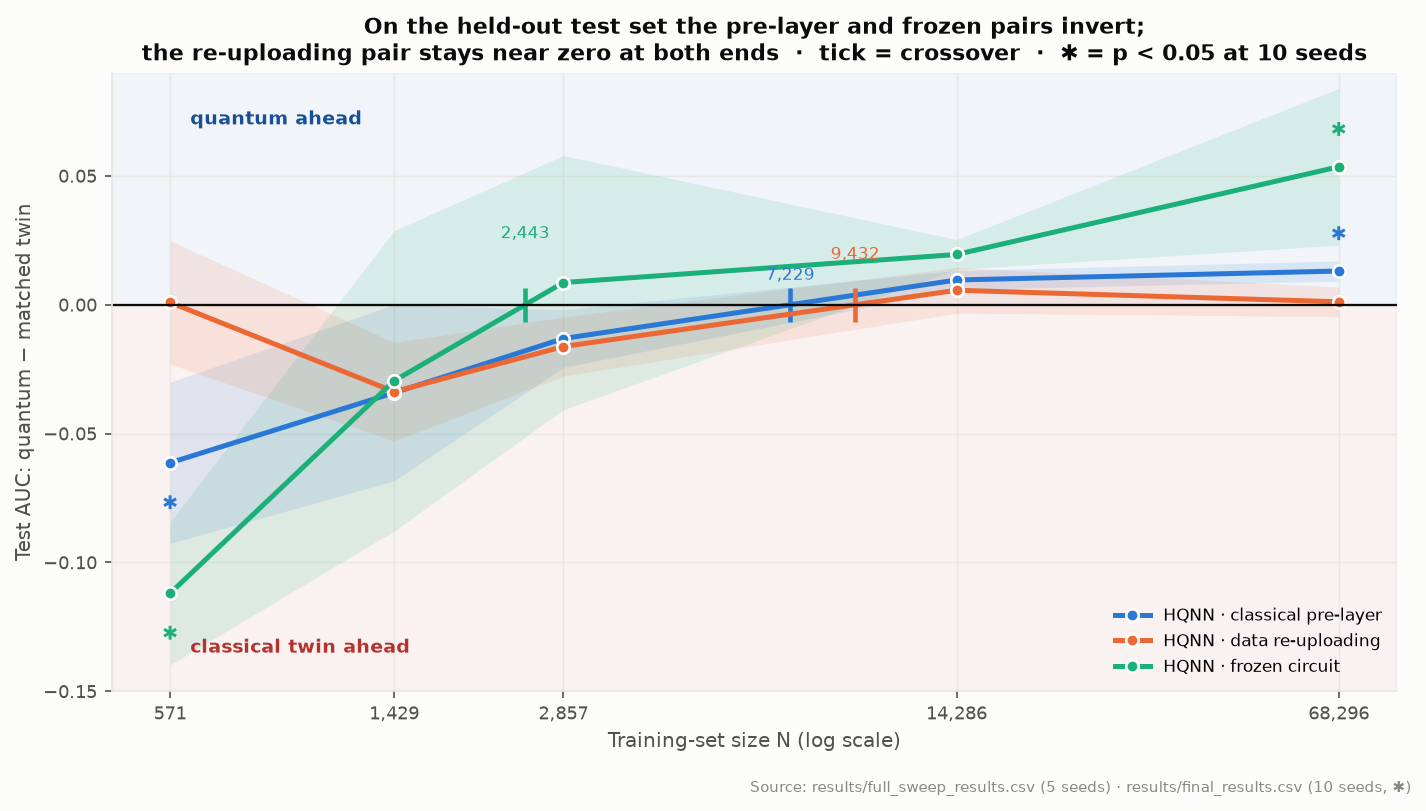
\includegraphics[width=\columnwidth]{19_inversion_test.png}
  \caption{Test AUC of each hybrid quantum network minus its matched classical
  twin, across five training-set sizes. Ticks mark the measured crossovers;
  stars mark comparisons significant at $p<0.05$ over 10 paired seeds. The
  pre-layer and frozen pairs invert; the re-uploading pair stays near zero.}
  \label{fig:inversion}
\end{figure}

\begin{figure}[t]
  \centering
  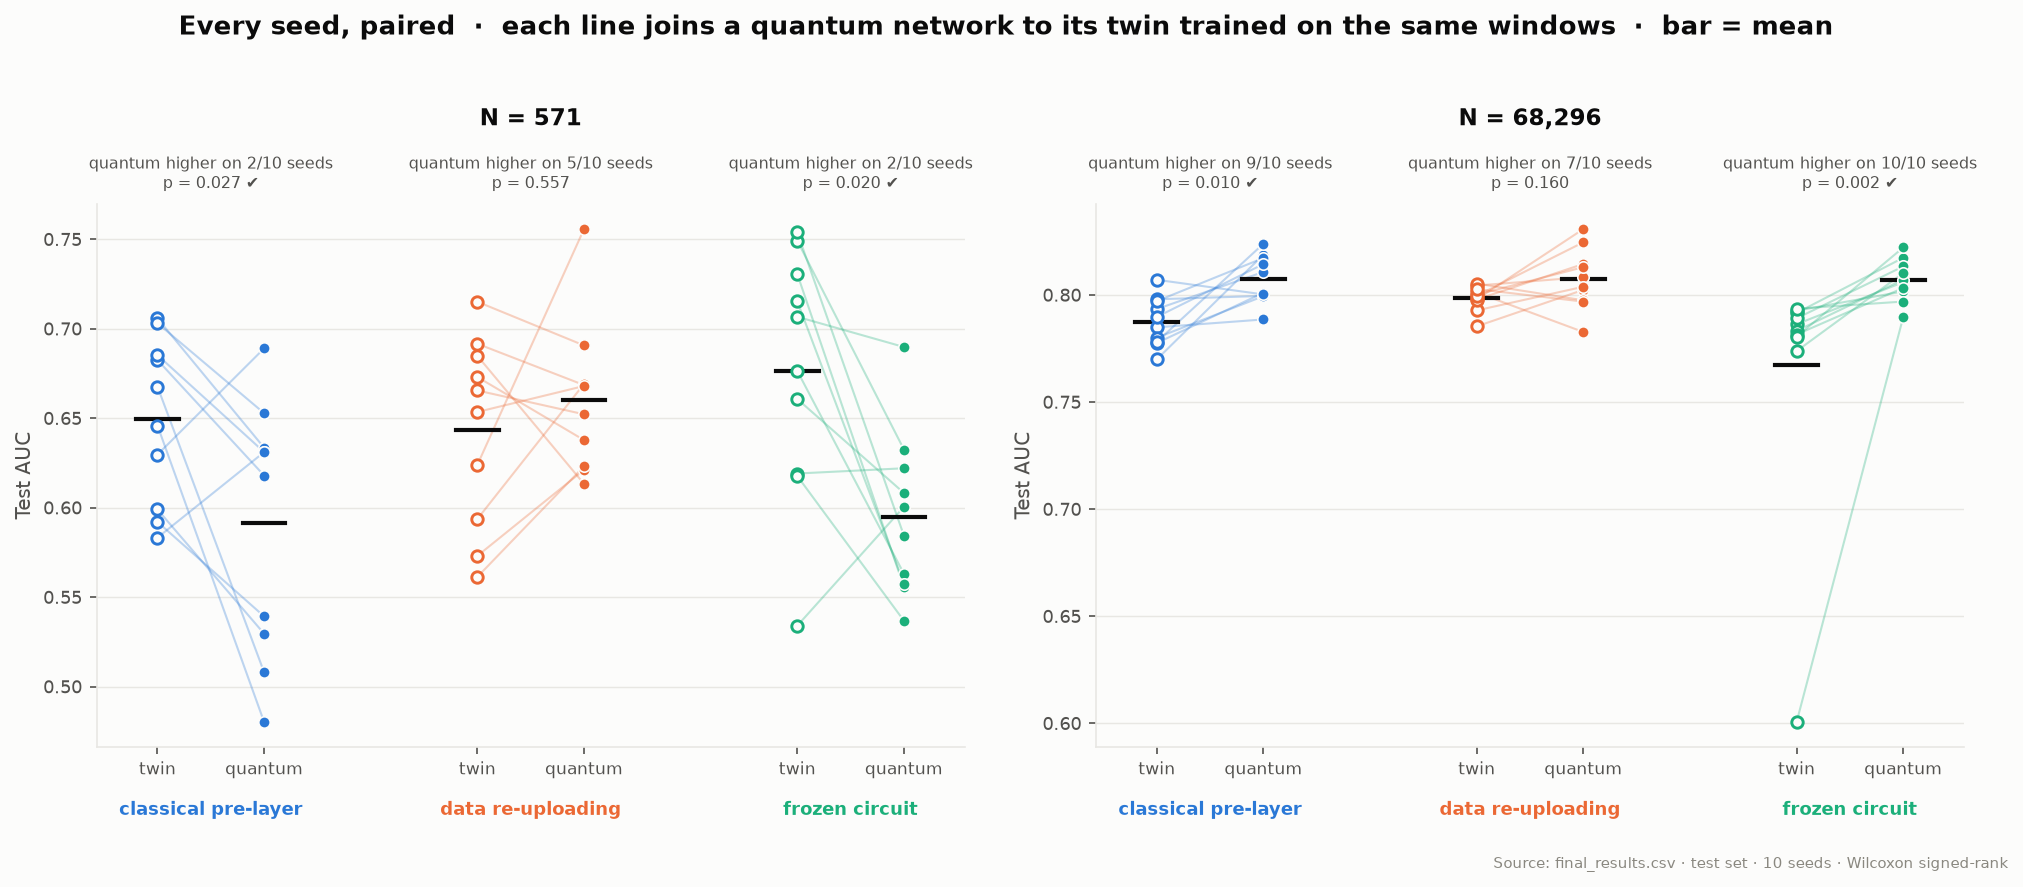
\includegraphics[width=\columnwidth]{10_endpoint_seeds.png}
  \caption{Every paired seed at both endpoints. Each line joins a quantum
  network to the classical twin trained on identical windows.}
  \label{fig:seeds}
\end{figure}

\begin{figure}[t]
  \centering
  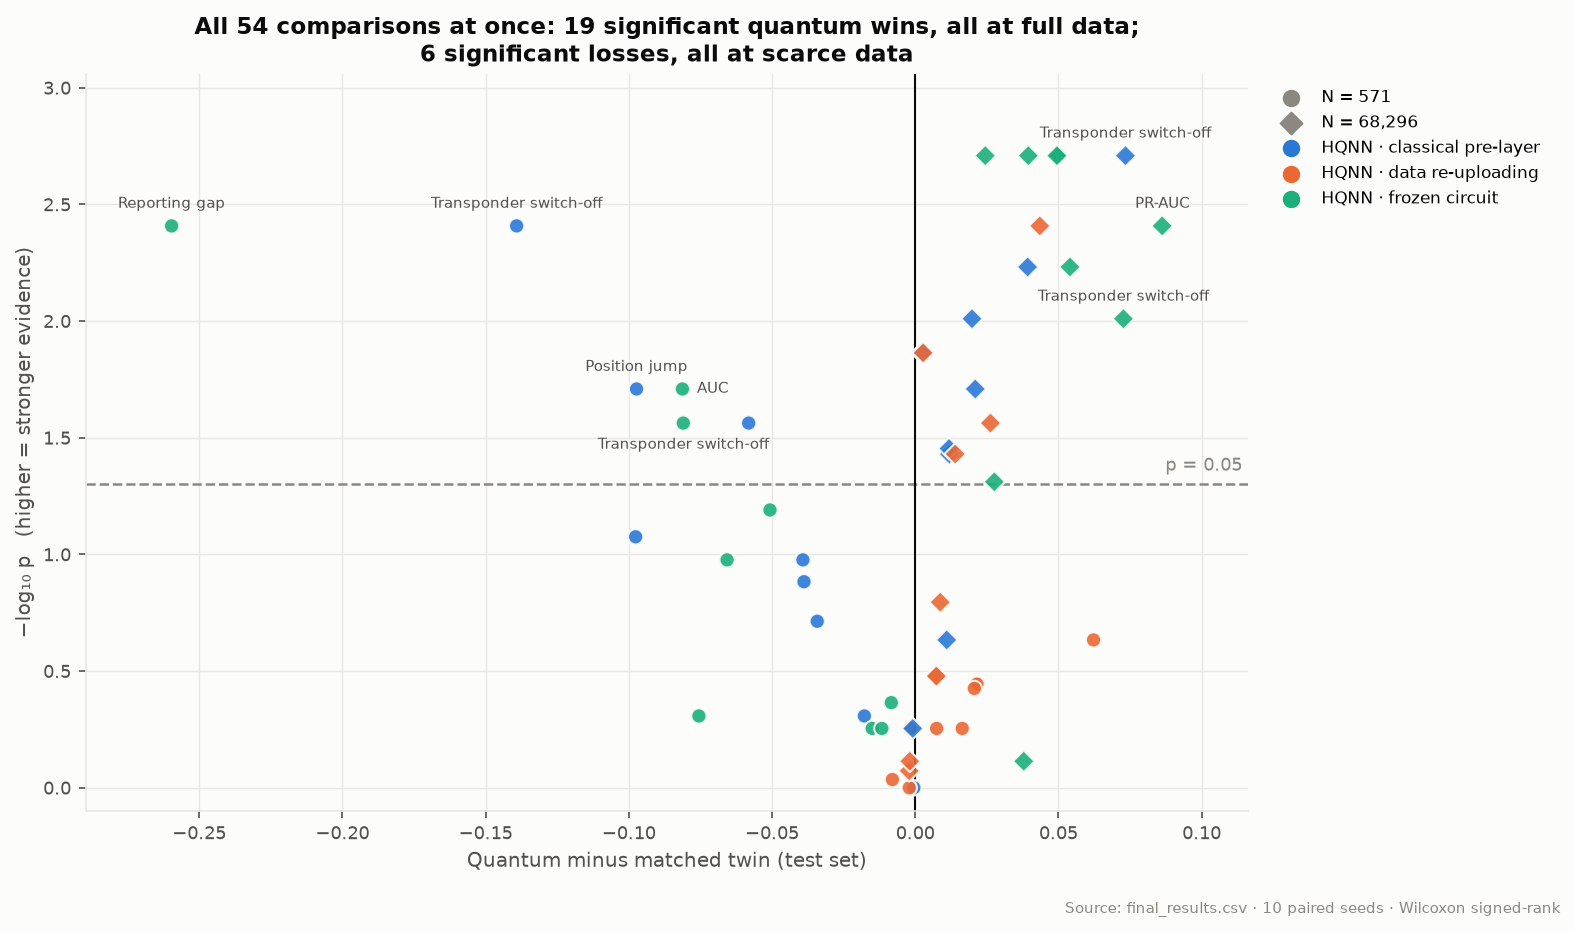
\includegraphics[width=\columnwidth]{12_significance_map.png}
  \caption{All 54 paired comparisons. Every significant quantum win occurs at
  full training data; every significant loss occurs when data are scarce.}
  \label{fig:significance}
\end{figure}

\subsection{Quantum Against the Best Classical Models}
\label{sec:sq2}
No quantum model outperforms the strongest classical models at any training-set
size (Table~\ref{tab:testauc}, Fig.~\ref{fig:ranking}). The gap between the best
quantum and the best classical model narrows from 0.119 at 571 windows (the
re-uploading network at 0.653 against random forest at 0.772) to 0.020 at
14,286 windows, then stops narrowing (0.026 at 68,296). At full data, gradient
boosting reaches 0.832 and random forest 0.823, against 0.807 for each of the
three quantum networks (ten seeds); on PR-AUC the gap is wider, 0.431--0.434
against 0.374--0.384. The quantum networks are level with logistic regression
(0.802) and the 71-parameter MLP (0.804): their margins over these models,
0.003--0.006, are smaller than their own seed-to-seed standard deviations,
0.010--0.014. Because that MLP has fewer parameters than any quantum network,
the results support no claim of parameter efficiency.

With little data, non-neural models outperform every neural network, quantum or
classical. At 571 windows the best non-neural model (isolation forest,
validation AUC 0.835) leads the best neural model (the frozen-circuit twin,
0.681) by 0.154, and the shortfall is shared by quantum and classical networks
alike. The isolation forest, which uses no labels, matches logistic regression
trained on 20 labeled anomalies (0.8349 against 0.8348).

\begin{figure}[t]
  \centering
  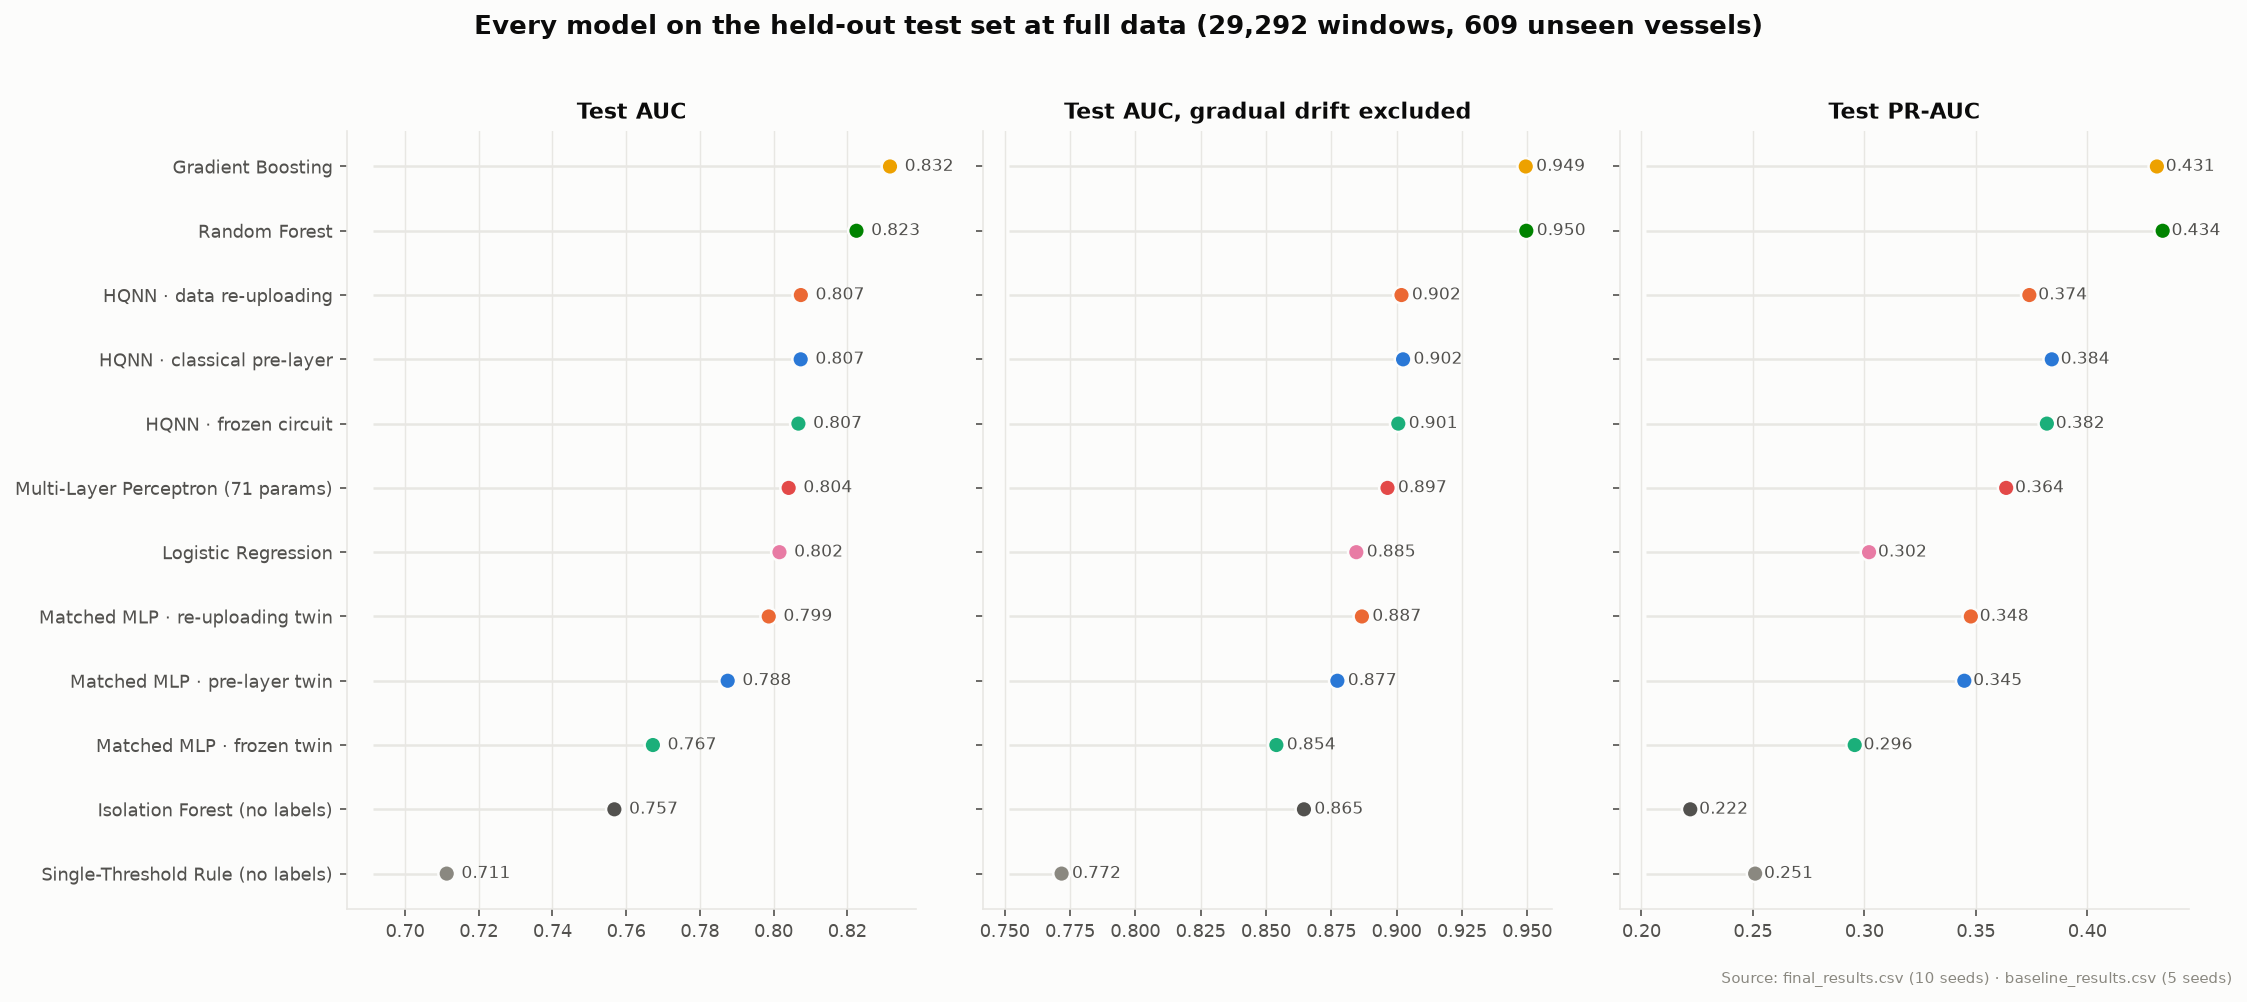
\includegraphics[width=\columnwidth]{13_model_ranking.png}
  \caption{Every model on the held-out test set at full training data: AUC,
  AUC with gradual drift excluded, and PR-AUC.}
  \label{fig:ranking}
\end{figure}

\subsection{Quantum Kernels Against Variational Circuits}
\label{sec:sq3}
The quantum kernel behaves differently from the variational circuits
(Fig.~\ref{fig:kernel}). At 571 windows it reaches a validation AUC of
$0.758\pm0.028$ and outperforms all seven neural networks, quantum and
classical, which range from 0.539 to 0.681; the best variational quantum network
reaches 0.624. It then barely improves: by $+0.005$ from 571 to 1,429 windows,
against $+0.117$ to $+0.128$ for the three variational quantum networks. By
1,429 windows two classical networks overtake it (the 71-parameter MLP at 0.803
and the re-uploading twin at 0.783), and the best non-neural classical models
exceed it at both sizes (0.835 and 0.855). Fig.~\ref{fig:curves} shows the full
learning curves on the test set.

The kernel model solves a convex problem: the circuit is fixed and the support
vector machine has a unique optimum. The variational networks are trained by
gradient descent over a non-convex landscape. That the kernel holds up with
scarce data while every variational quantum network collapses indicates that
the quantum models' scarce-data deficit lies in training variational circuits,
not in quantum feature maps as such.

\begin{figure}[t]
  \centering
  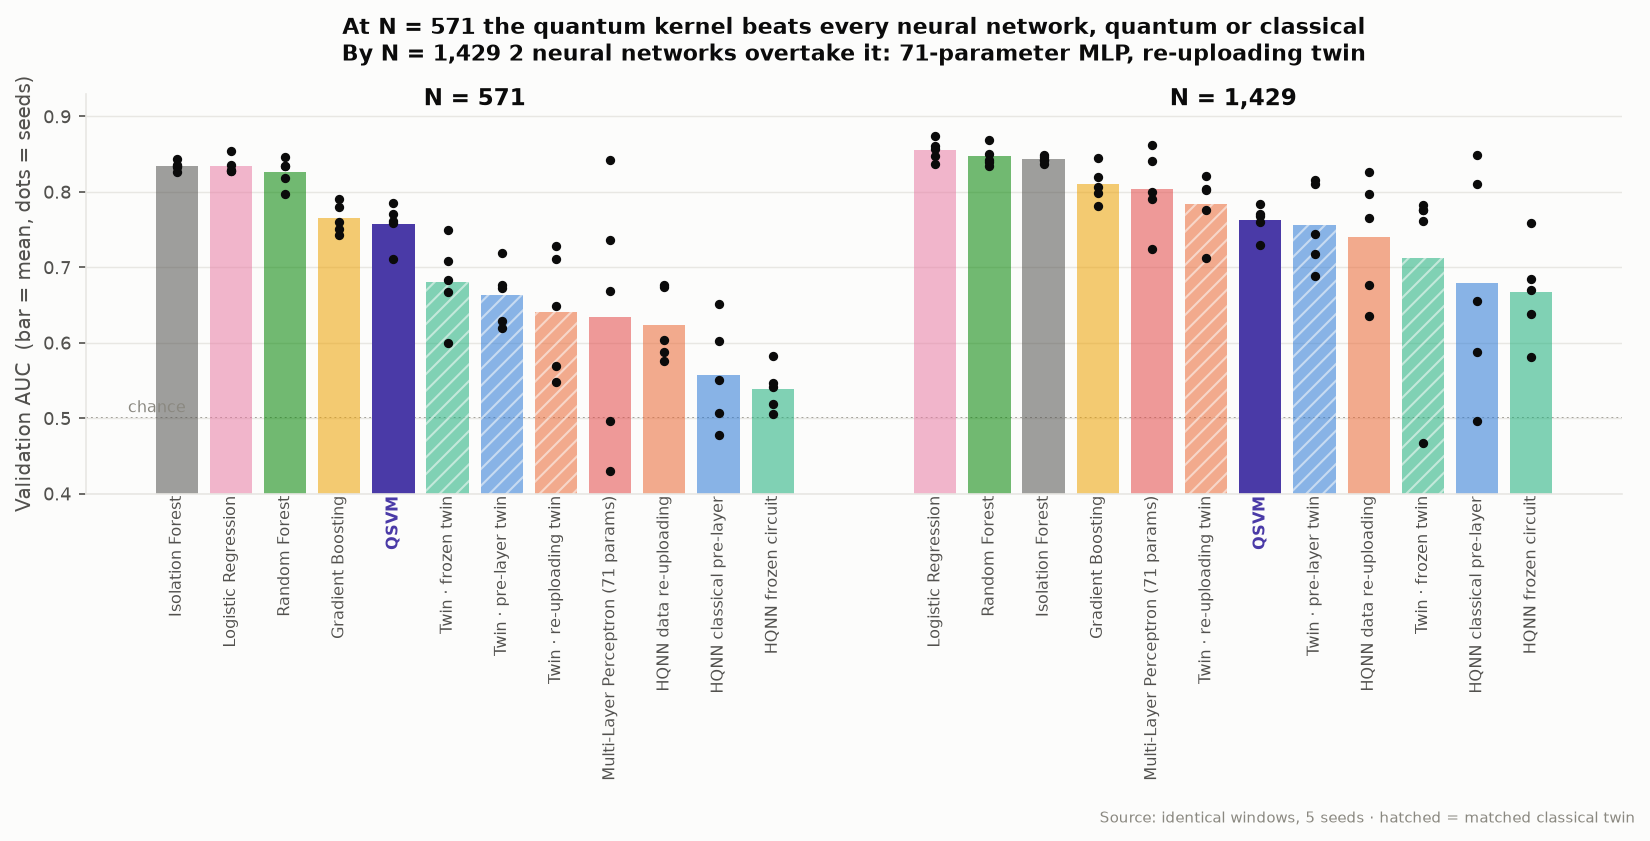
\includegraphics[width=\columnwidth]{14_quantum_kernel.png}
  \caption{The quantum kernel against every other model at the two smallest
  training-set sizes (validation AUC, five seeds).}
  \label{fig:kernel}
\end{figure}

\begin{figure*}[t]
  \centering
  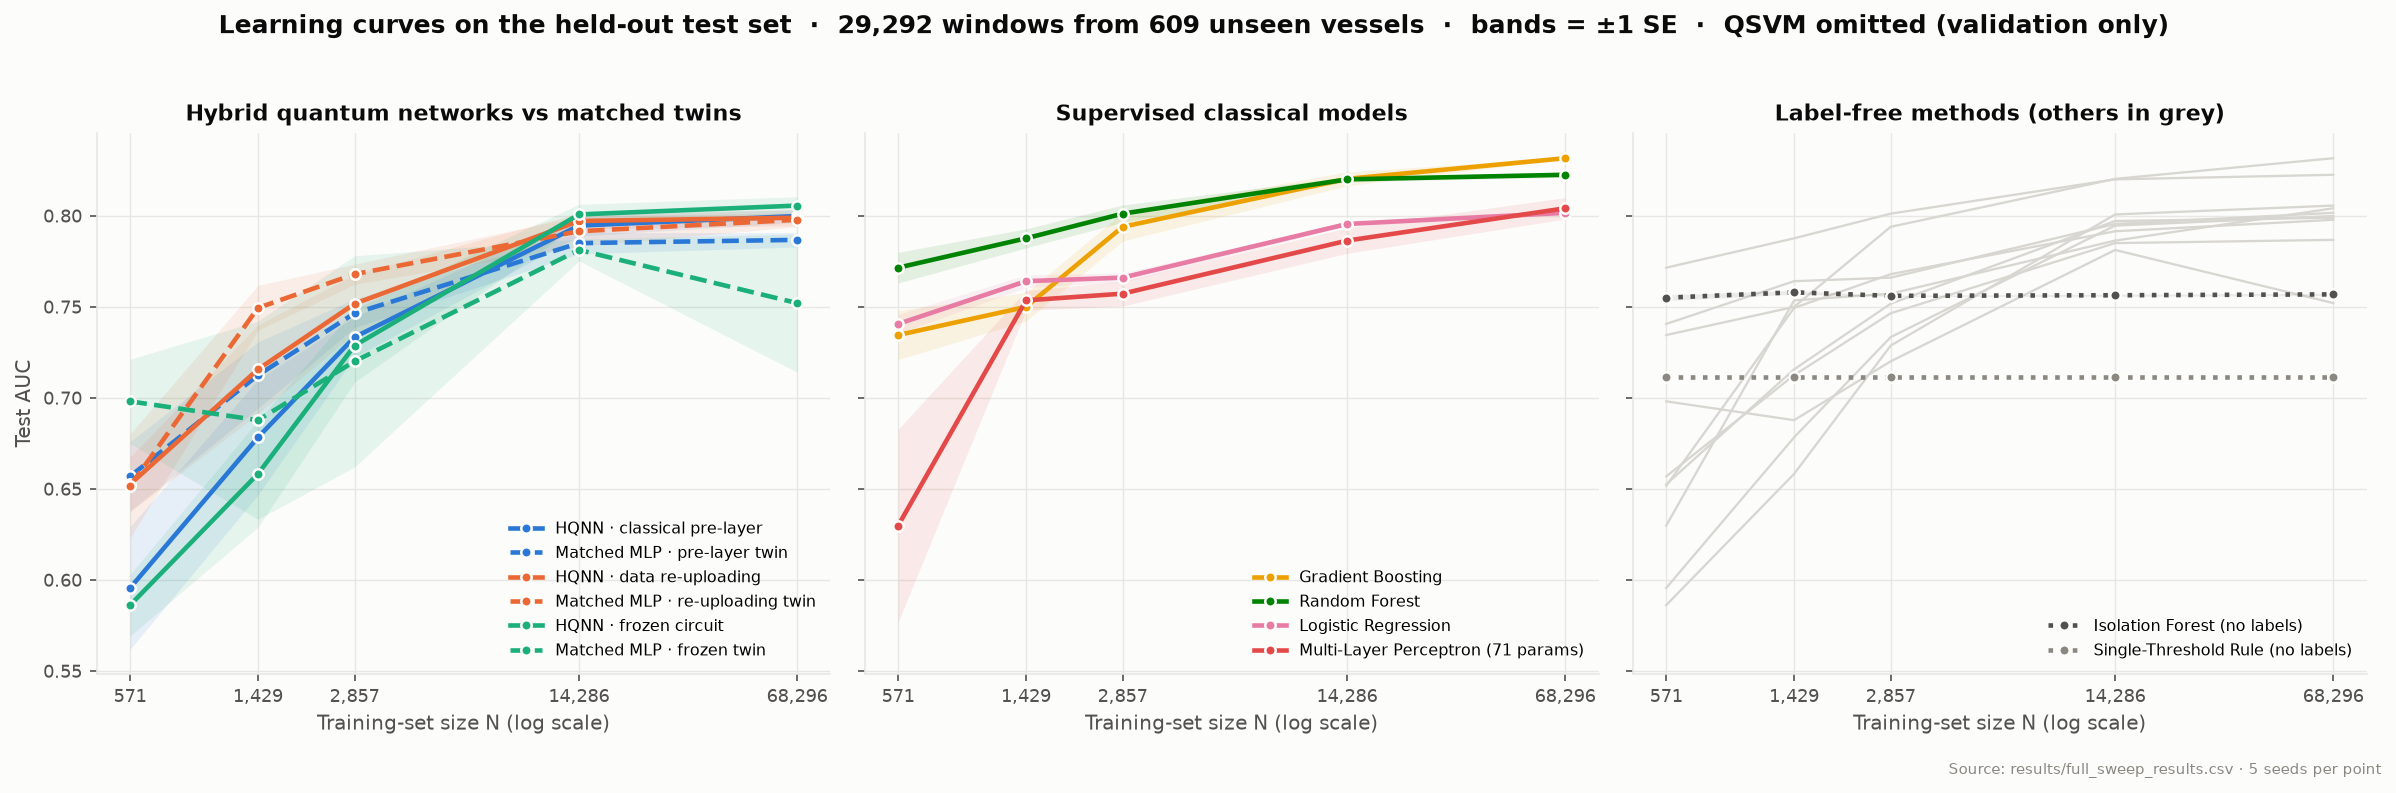
\includegraphics[width=\textwidth]{18_learning_curves_test.png}
  \caption{Learning curves on the held-out test set (29,292 windows from 609
  vessels never seen in training), with the anomaly rate held at 3.5\%. Bands
  are one standard error over five seeds. The quantum kernel is omitted because
  it was scored on validation only; its results are in Fig.~\ref{fig:kernel}.}
  \label{fig:curves}
\end{figure*}

\subsection{A Measured Ceiling, and Quantum Features in Tree Models}
\label{sec:sq4}

\subsubsection{Geometric difference}
Following Huang \textit{et al.}~\cite{huang2021power}, we computed the geometric
difference $g$ between the QSVM's quantum kernel and eight classical kernels
(Gaussian kernels at seven bandwidths spanning a 1,000-fold range, and a linear
kernel) on the same subsamples and inputs, counting only classical kernels able
to fit the training data. The value of $g$ lies between 1 and $\sqrt{N}$, and a
classical kernel can learn any function the quantum kernel can with at most
$g^2$ times its model complexity. The median $g$ over five seeds is 2.9 at 571
windows and 3.8 at 1,429, against maxima of 23.9 and 37.8
(Table~\ref{tab:geometric}, Fig.~\ref{fig:geometric}): about 12\% and 10\% of
the largest possible separation. The room for a quantum-kernel advantage on
these data is therefore small, and it shrinks relative to its maximum as the
data grow.

On the actual labels, the quantum kernel is the simpler description at
571 windows: with ridge parameter 0.01, its model complexity is lower than that
of every fitting classical kernel on five of five seeds. The advantage does not
persist. At 1,429 windows, with ridge parameter 0.001, where classical kernels
fit on every seed, the quantum kernel is the more complex description on five of
five seeds.

\subsubsection{Quantum features in tree ensembles}
We also tested whether features computed by a quantum circuit improve the tree
ensembles used in practice. The single-qubit expectation values $\langle
X_i\rangle$, $\langle Y_i\rangle$ and $\langle Z_i\rangle$ of the QSVM's
IQP-embedded state gave 16 non-constant features; every $\langle Z_i\rangle$
vanishes for a single IQP repetition. Random forest and gradient boosting, with
their tuned settings, were trained on the twelve original features alone, with
the 16 quantum features added, and with three classical controls computed from
the same eight inputs: 16 random Fourier features, 16 random $\tanh$ features,
and the eight inputs themselves. Five sizes, ten seeds, five input sets and two
models gave 500 fits (Fig.~\ref{fig:qfeatures}, Table~\ref{tab:qfeatures}).

Quantum features lowered test AUC in all ten model-and-size combinations, and
significantly for random forest at every size ($-0.010$ to $-0.024$,
$p\le 0.004$). They were never better than the best classical control,
outperforming random Fourier features once (gradient boosting at 571 windows,
$p=0.037$).

\subsubsection{The validation/test reversal}
On the validation set, random forest with quantum features outperformed both the
plain model and every classical control at the two largest sizes ($+0.006$ to
$+0.010$, $p\le 0.049$). On the test set the same comparison reversed: at 68,296
windows the quantum features lowered AUC by 0.010 ($p=0.002$). The two sets
contain different vessels, and an effect that changes sign between them is not
a property of the model. Had only the validation set been examined, this result
would have been reported as a quantum advantage.

\begin{figure*}[t]
  \centering
  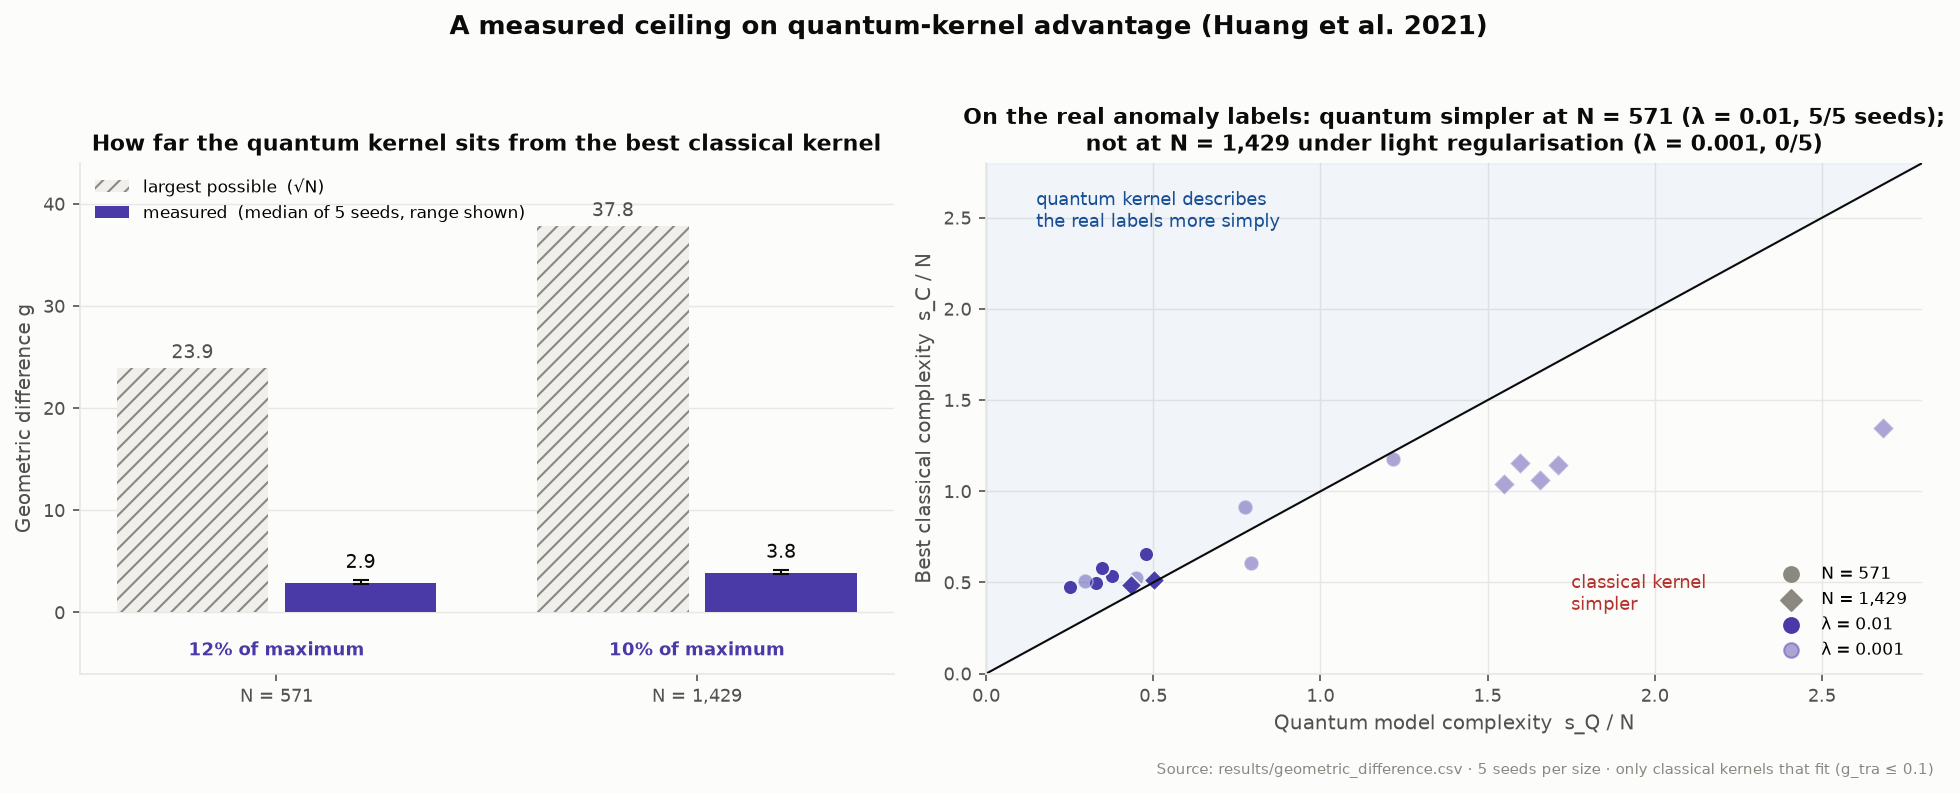
\includegraphics[width=\textwidth]{20_geometric_difference.png}
  \caption{Left: the geometric difference between the quantum kernel and the
  best classical kernel able to fit the data, against the largest value it
  could take. Right: model complexity on the real anomaly labels; points above
  the diagonal are where the quantum kernel describes the labels more simply.}
  \label{fig:geometric}
\end{figure*}

\begin{figure*}[t]
  \centering
  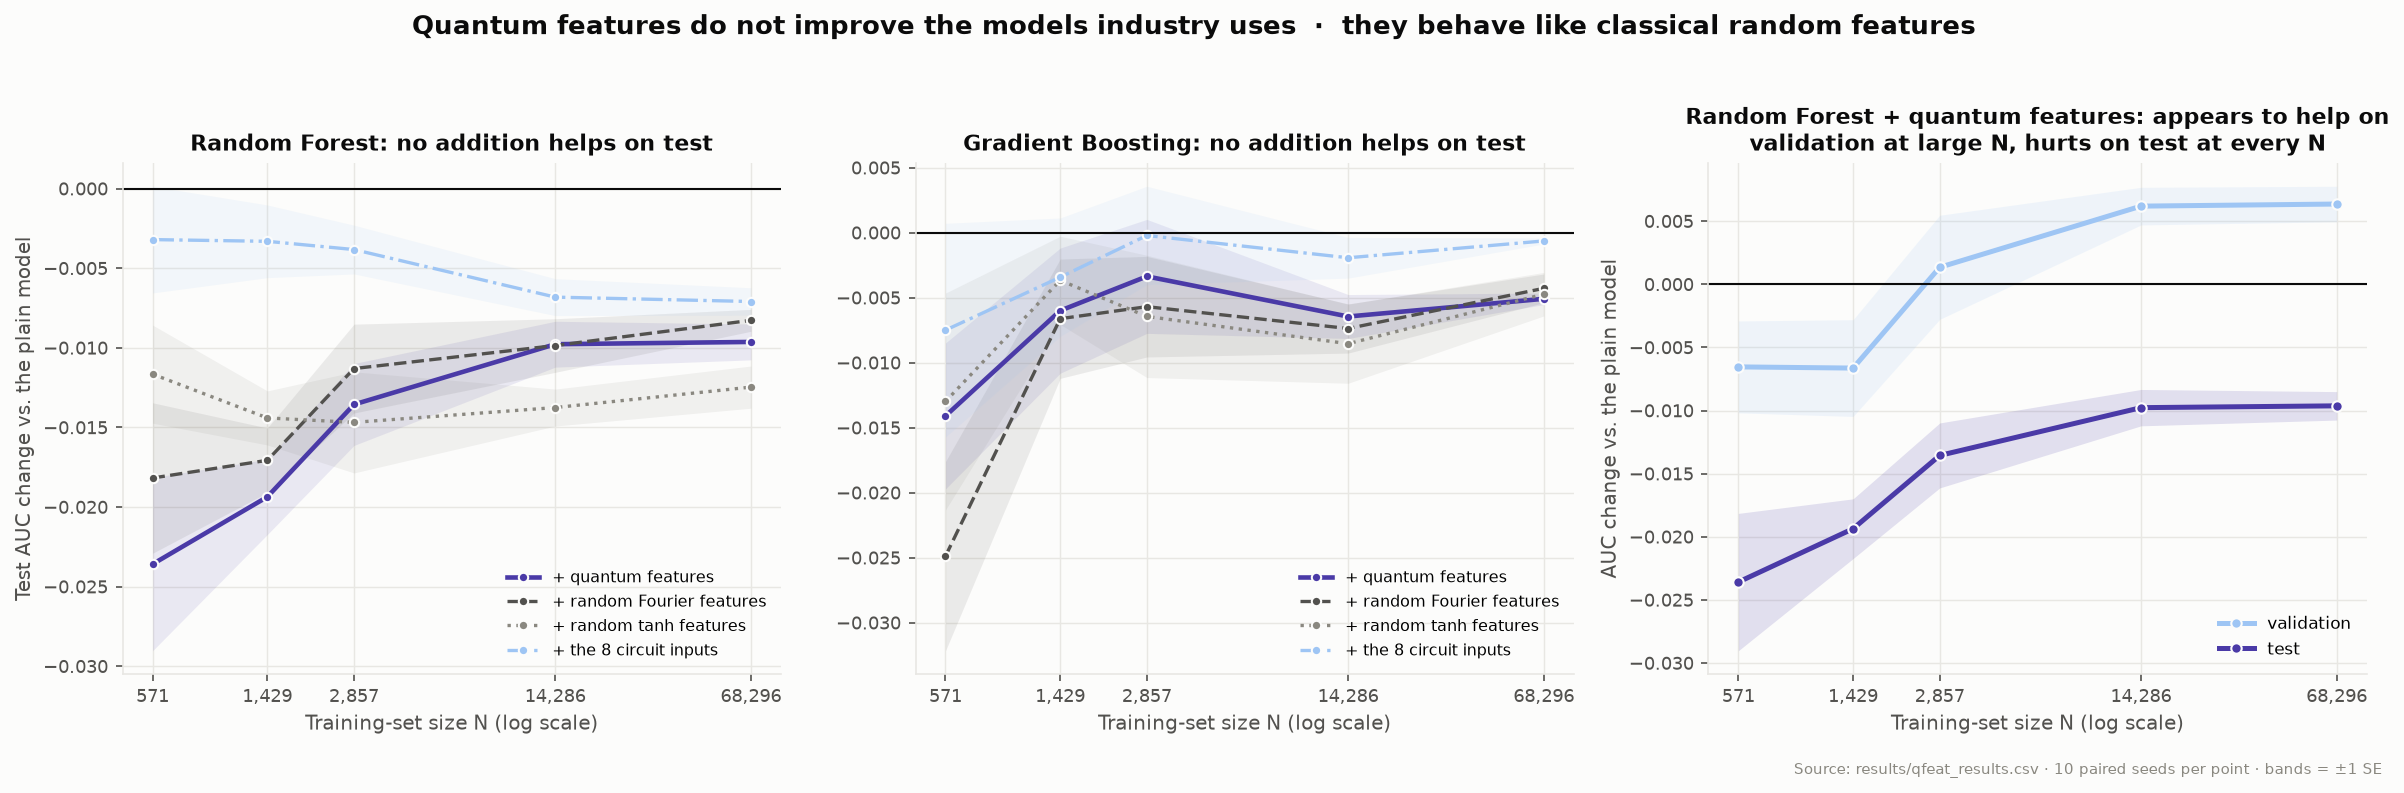
\includegraphics[width=\textwidth]{21_quantum_features.png}
  \caption{Quantum features added to random forest and gradient boosting,
  against three classical controls computed from the same eight inputs (left,
  center). Right: for random forest the quantum features appear to help on
  validation at large training sizes but lower AUC on the held-out test set at
  every size.}
  \label{fig:qfeatures}
\end{figure*}

% GENERATED by scripts/27_paper_tables.py -- do not edit by hand
\begin{table}[t]
\centering
\caption{Geometric difference between the quantum kernel and the best classical kernel that can fit the data, against the largest value it could take. A classical kernel can learn any function the quantum kernel can, at no more than $g^{2}$ times the model complexity.}
\label{tab:geometric}
\begin{tabular}{lrrr}
\toprule
Quantity & $g$ & $\sqrt{N}$ & Share of maximum \\
\midrule
Geometric difference{,} $N{=}571$ & $2.91$ & $23.9$ & 12\% \\
Geometric difference{,} $N{=}1{,}429$ & $3.83$ & $37.8$ & 10\% \\
\bottomrule
\end{tabular}
\end{table}

% GENERATED by scripts/27_paper_tables.py -- do not edit by hand
\begin{table}[t]
\centering
\footnotesize
\setlength{\tabcolsep}{4pt}
\caption{Quantum features added to the two strongest classical models, against the plain model and against classical random features of the same count. Negative means the quantum features made the model worse. Ten paired seeds, test set.}
\label{tab:qfeatures}
\begin{tabular}{lrr}
\toprule
Model and size & vs.\ plain & vs.\ random features \\
\midrule
Random forest{,} $N{=}571$ & $-0.0236$$^{*}$ & $-0.0054$ \\
Random forest{,} $N{=}68{,}296$ & $-0.0096$$^{*}$ & $-0.0014$ \\
Gradient boosting{,} $N{=}571$ & $-0.0141$$^{*}$ & $+0.0108$$^{*}$ \\
Gradient boosting{,} $N{=}68{,}296$ & $-0.0051$$^{*}$ & $-0.0008$ \\
\bottomrule
\end{tabular}
\\[2pt]\footnotesize $^{*}$ $p<0.05$, Wilcoxon signed-rank.
\end{table}


\subsection{Detection by Attack Type}
\label{sec:attacks}
Fig.~\ref{fig:perattack} breaks test AUC down by attack type at full data, with
ten paired seeds; Table~\ref{tab:attacks} gives five-seed values for every
model. The quantum networks' largest advantage over their twins is on
transponder switch-off: $+0.073$ for the pre-layer network (0.819 against 0.746,
$p=0.002$) and for the frozen circuit (0.814 against 0.741, $p=0.010$), and
$+0.044$ for the re-uploading network ($p=0.004$). This is the attack most
closely associated with concealed fishing activity~\cite{welch2022unseen}; the
tree ensembles nonetheless remain far ahead on it, at 0.961. On speed
falsification, the re-uploading network reaches 0.998, the highest score of any
model on any attack, against 0.994 for gradient boosting, although every model
is close to the ceiling there. All three quantum networks also significantly
outperform their twins on reporting gaps ($+0.014$ to $+0.024$).

Gradual drift, 37.7\% of test anomalies, remains unsolved. Every supervised
model scores between 0.61 and 0.66 on it, the threshold rule 0.61, and the
isolation forest 0.58. Because drift leaves speed, course and heading unchanged
and accumulates slowly, it produces no abrupt change for maximum-based features
to detect.

\begin{figure*}[t]
  \centering
  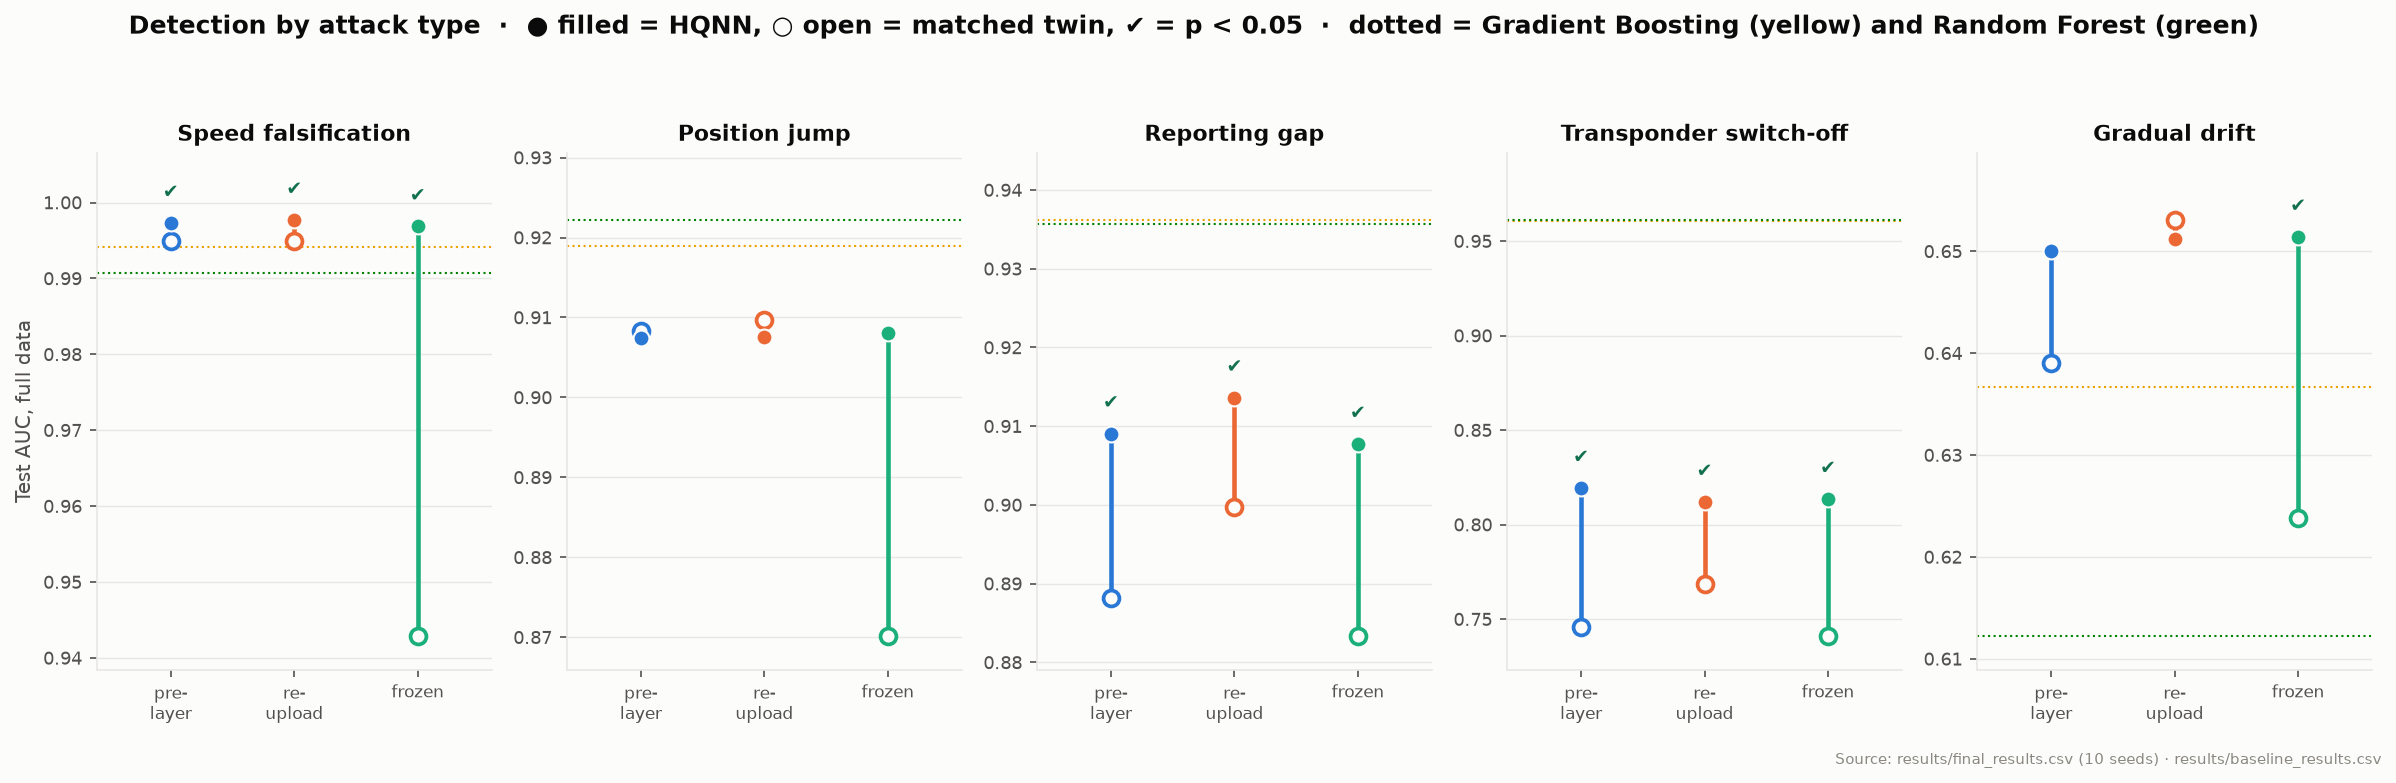
\includegraphics[width=\textwidth]{11_attack_detection.png}
  \caption{Detection by attack type at full training data, ten paired seeds.
  Filled markers are the hybrid quantum networks and open markers their matched
  twins; dotted lines are gradient boosting and random forest.}
  \label{fig:perattack}
\end{figure*}

% GENERATED by scripts/27_paper_tables.py -- do not edit by hand
\begin{table*}[t]
\centering
\caption{Test AUC for every model at every training-set size. Five seeds per cell, identical training windows across models. Bold marks the best model at that size. The quantum kernel has validation scores only and is reported separately.}
\label{tab:testauc}
\begin{tabular}{lrrrrr}
\toprule
Model & $N{=}571$ & $N{=}1{,}429$ & $N{=}2{,}857$ & $N{=}14{,}286$ & $N{=}68{,}296$ \\
\midrule
HQNN, data re-uploading & 0.6525 & 0.7156 & 0.7517 & 0.7971 & 0.7989 \\
HQNN, classical pre-layer & 0.5956 & 0.6783 & 0.7333 & 0.7946 & 0.7998 \\
HQNN, frozen circuit (control) & 0.5861 & 0.6582 & 0.7287 & 0.8007 & 0.8056 \\
Quantum SVM & --- & --- & --- & --- & --- \\
Gradient boosting & 0.7345 & 0.7499 & 0.7939 & \textbf{0.8202} & \textbf{0.8316} \\
Random forest & \textbf{0.7715} & \textbf{0.7876} & \textbf{0.8011} & 0.8200 & 0.8225 \\
Logistic regression & 0.7406 & 0.7640 & 0.7660 & 0.7955 & 0.8016 \\
MLP (12-5-1, 71 par.) & 0.6298 & 0.7535 & 0.7572 & 0.7863 & 0.8041 \\
Twin of re-uploading HQNN & 0.6516 & 0.7494 & 0.7679 & 0.7915 & 0.7978 \\
Twin of pre-layer HQNN & 0.6569 & 0.7124 & 0.7464 & 0.7850 & 0.7867 \\
Twin of frozen HQNN & 0.6981 & 0.6877 & 0.7201 & 0.7812 & 0.7520 \\
Isolation forest (no labels) & 0.7550 & 0.7579 & 0.7560 & 0.7563 & 0.7568 \\
Threshold rule (no labels) & 0.7113 & 0.7113 & 0.7113 & 0.7113 & 0.7113 \\
\bottomrule
\end{tabular}
\end{table*}

% GENERATED by scripts/27_paper_tables.py -- do not edit by hand
\begin{table*}[t]
\centering
\caption{Test AUC by attack type at full training data. Bold marks the best model for that attack. Gradual drift, the largest attack class, is unsolved by every model.}
\label{tab:attacks}
\begin{tabular}{lrrrrr}
\toprule
Model & Speed falsif. & Position jump & Reporting gap & Transponder off & Gradual drift \\
\midrule
HQNN, data re-uploading & \textbf{0.997} & 0.908 & 0.917 & 0.799 & 0.633 \\
HQNN, classical pre-layer & \textbf{0.997} & 0.907 & 0.907 & 0.787 & 0.645 \\
HQNN, frozen circuit (control) & 0.997 & 0.905 & 0.909 & 0.805 & 0.653 \\
Gradient boosting & 0.994 & 0.919 & \textbf{0.936} & 0.961 & 0.637 \\
Random forest & 0.991 & \textbf{0.922} & \textbf{0.936} & \textbf{0.961} & 0.612 \\
Logistic regression & 0.988 & 0.908 & 0.887 & 0.780 & \textbf{0.664} \\
MLP (12-5-1, 71 par.) & 0.994 & 0.908 & 0.890 & 0.818 & 0.651 \\
Twin of re-uploading HQNN & 0.993 & 0.913 & 0.895 & 0.750 & 0.660 \\
Twin of pre-layer HQNN & 0.995 & 0.908 & 0.899 & 0.732 & 0.638 \\
Twin of frozen HQNN & 0.892 & 0.832 & 0.885 & 0.717 & 0.627 \\
Isolation forest (no labels) & 0.926 & 0.911 & 0.869 & 0.765 & 0.579 \\
Threshold rule (no labels) & 0.971 & 0.909 & 0.714 & 0.539 & 0.611 \\
\bottomrule
\end{tabular}
\end{table*}


%------------------------------------------------------------------ discussion
\section{Discussion}
\label{sec:discussion}
% DRAFT -- rewrite in your own words before submission.

\subsection{Optimization, Not Generalization}
The central result runs opposite to the common reading of the generalization
bound, but it does not contradict the bound. Caro
\textit{et al.}~\cite{caro2022generalization} bound the gap between training and
test error; a model that cannot fit its training data has a small gap and still
performs poorly. Three observations point to optimization as the binding
constraint at small $N$. First, the quantum kernel, which involves no circuit
training, does not collapse. Second, freezing the 48 quantum angles changes
nothing measurable, so the trainable quantum gates are the source of neither the
small-data deficit nor the full-data advantage. Third, the classical twins,
trained with the same step budget, also degrade with scarce data, but less than
the pre-layer and frozen-circuit networks. This is consistent with Gil-Fuster
\textit{et al.}~\cite{gilfuster2024rethinking}, who show that uniform
generalization bounds cannot by themselves explain how quantum models behave,
and with the known difficulty of training variational
circuits~\cite{cerezo2021vqa,larocca2025barren}. We did not measure gradient
variance, so we cannot attribute the deficit to barren plateaus specifically.

Because the frozen circuit matches the trained one, the full-data advantage over
the twins appears to come from combining a trained classical layer with a fixed
quantum feature map, which then functions much like a random-feature model.
That the quantum features of Section~\ref{sec:sq4} behaved no better than
classical random features in tree models is consistent with this reading.

\subsection{What the Size Constraint Means in Practice}
The quantum advantage of Section~\ref{sec:sq1} holds only when the classical
model is restricted to the same size, depth and training schedule. No
operational detector would impose that restriction, and without it gradient
boosting outperforms every quantum model. The constraint is not wholly
artificial: detectors running aboard satellites or buoys that receive AIS have
tight memory and power budgets. Even there, however, the 71-parameter MLP
matched the quantum networks, so the comparison favors quantum models only
against twins trained under an identical schedule, not against small classical
models in general.

\subsection{Where Quantum Advantage Is Proven, and Why AIS Is Not There}
Provable quantum advantages in learning rely on data with special structure or
on data that are themselves quantum. Liu \textit{et al.}~\cite{liu2021rigorous}
prove an advantage for a classification problem built on the discrete
logarithm, and Huang \textit{et al.}~\cite{huang2022experiments} demonstrate one
when the data come from quantum experiments. For classical data, Huang, Kueng
and Preskill~\cite{huang2021information} show that quantum models can offer at
most a polynomial advantage in sample complexity for average-case prediction,
and Tang~\cite{tang2019quantum} showed that a claimed exponential quantum
speed-up on classical data could be matched by a classical algorithm. AIS
reports are classical, low-dimensional and without a known group structure. The
measured geometric difference, about a tenth of its maximum and shrinking
relative to it, is consistent with that picture.

\subsection{Operational Significance}
Two results bear on practice. The quantum networks' largest gain over their
twins falls on transponder switch-off, the attack most associated with concealed
activity at sea, but tree ensembles detect that attack far better. And the
validation/test reversal in the quantum-feature experiment shows how easily a
quantum advantage can be reported in error: random forest with quantum features
appeared to beat every classical control on one set of vessels and lost to the
plain model on another. Evaluating on held-out vessels against paired controls
is what prevented that error.

%----------------------------------------------------------------- limitations
\section{Limitations}
\label{sec:limitations}
% DRAFT -- rewrite in your own words before submission.
All quantum models used eight qubits, one encoding scheme per model family, and
noiseless simulation; we report no results from quantum hardware, where noise
would be expected to lower performance. Every HQNN compresses twelve features
into eight through a classical layer, while its twin reads all twelve. We
measured neither runtime nor parameter efficiency and claim no advantage in
either; a 71-parameter classical network matched the 106--161-parameter quantum
models.

The anomalies were injected, not observed, and real manipulation may differ from
the five attacks modeled here. The data cover a single day of United States
coastal AIS, so we make no seasonal or geographic claim. Gradual drift, the
largest attack class, was not solved by any model.

The quantum models and their twins were tuned over two configurations each,
whereas the classical baselines were tuned over 9--12, which favors the
baselines. The twin of the frozen circuit was unstable across seeds, with a test
AUC standard deviation of 0.059 at full data. The test set was scored by several
experiments, although no setting was ever chosen on it. Median imputation of
missing feature values used statistics computed over all windows before the
split; no labels were involved. The robustness rebuilds of
Appendix~\ref{app:repro} were run on an earlier, seven-feature version of the
dataset. The QSVM was evaluated on validation data only, and only at 571 and
1,429 windows.

%----------------------------------------------------------------- future work
\section{Future Work}
\label{sec:future}
% DRAFT -- rewrite in your own words before submission.
The most direct next experiment is to retrain the variational networks with the
quantum natural gradient~\cite{stokes2020qng}, which accounts for the geometry
of the quantum state space. If the scarce-data deficit is an optimization
problem, it should narrow. A second is to use twelve or more qubits, removing the
compression that the current networks require. Third, covariant quantum kernels,
built around a symmetry group in the data~\cite{glick2024covariant}, could
exploit the rotational and translational symmetries of vessel tracks, which the
IQP feature map ignores. Fourth, quantum advantage is best supported when the
data are themselves quantum~\cite{huang2022experiments}; quantum sensors being
developed for navigation could eventually supply such data to maritime
monitoring. Sequence models such as quantum long short-term memory
networks~\cite{chen2022qlstm}, and tree-based quantum models such as quantum
random forests~\cite{srikumar2024qrf}, were not tested here. Finally, the
contrasting learning curves suggest a hybrid detector that uses a quantum kernel
where confirmed anomalies are few and switches to other models as labels
accumulate, although in our data simple classical models outperformed both in
that regime.

%------------------------------------------------------------------ conclusion
\section{Conclusion}
\label{sec:conclusion}
% DRAFT -- rewrite in your own words before submission.
We asked under what conditions quantum machine learning models outperform
classical models in detecting anomalous vessel behavior in AIS data. Against
classical networks of equal size and depth, trained on identical data with the
same number of optimization steps, hybrid quantum networks perform worse when
labeled data are scarce and better when they are plentiful, with the crossover
at a few thousand training windows. This is the opposite of what a common
reading of quantum generalization bounds predicts, and our controls locate the
cause in the training of variational circuits rather than in quantum feature
maps. Against the classical models used in practice, no quantum model
outperformed gradient boosting or random forest at any training-set size, and
the room for any quantum-kernel advantage on these data is small. For maritime
surveillance as it stands, quantum machine learning offers no practical
advantage. The conditions under which it might, namely quantum-native data,
feature maps built on the structure of the problem, and better optimizers for
variational circuits, are what future work should test.

%--------------------------------------------------------------------- backmatter
\appendices

\section{Feature Definitions}
\label{app:features}
Each feature is computed over one window of ten consecutive reports from a
single voyage. Features marked $\dagger$ were added after an initial study showed
that maximum-based features could not detect gradual trends.

\begin{table}[!h]
\centering
\footnotesize
\setlength{\tabcolsep}{4pt}
\caption{The twelve features}
\label{tab:featdefs}
\begin{tabular}{@{}p{0.34\columnwidth}p{0.6\columnwidth}@{}}
\toprule
Feature & Definition \\
\midrule
\texttt{sog\_mean} & Mean reported speed over ground \\
\texttt{sog\_max\_jump} & Largest change in reported speed between consecutive reports \\
\texttt{cog\_turn\_max} & Largest change in reported course between consecutive reports \\
\texttt{dt\_max} & Longest interval between consecutive reports \\
\texttt{spd\_mismatch\_max} & Largest absolute difference between implied and reported speed \\
\texttt{crab\_mean} & Mean angle between reported course and reported heading \\
\texttt{prev\_silence\_s} & Silence preceding the window's voyage \\
\texttt{course\_resid\_mean}$^\dagger$ & Mean angle between reported course and the bearing travelled \\
\texttt{mismatch\_slope}$^\dagger$ & Least-squares slope of the speed mismatch across the window \\
\texttt{straightness}$^\dagger$ & Net displacement divided by path length \\
\texttt{mismatch\_mean}$^\dagger$ & Mean absolute difference between implied and reported speed \\
\texttt{crab\_valid} & 1 if heading was reported in the window, else 0 \\
\bottomrule
\end{tabular}
\end{table}

\section{Attack Injection Parameters}
\label{app:attacks}

\begin{table}[!h]
\centering
\footnotesize
\setlength{\tabcolsep}{4pt}
\caption{Injected attacks. Severities are drawn uniformly from each range;
medians are measured from the final dataset.}
\label{tab:attackparams}
\begin{tabular}{@{}lrrrr@{}}
\toprule
Attack & Range & Median & Voyages & Windows \\
\midrule
Speed falsification & $\times$1.8--5.0 & $\times$2.8 & 49 & 588 \\
Position jump & 0.5--20~km & 9.8~km & 595 & 714 \\
Reporting gap & 500--1,700~s & 1,093~s & 794 & 677 \\
Transponder switch-off & 1--6~h & 3.6~h & 1,091 & 681 \\
Gradual drift & 0.1--3~km & 1.3~km & 124 & 1,332 \\
\bottomrule
\end{tabular}
\end{table}

\section{Complete Results}
\label{app:results}
Table~\ref{tab:testauc} gives test AUC for every model at every training-set
size. Validation AUC, PR-AUC and per-attack AUC at every size, and every
individual run, are available in the repository, together with the script that
generates every table in this paper directly from the result files.

\section{Reproducibility}
\label{app:repro}
\textit{Software.} Python 3.13, PennyLane 0.45.1~\cite{bergholm2018pennylane}
with JAX 0.10.2 and Optax 0.2.8, scikit-learn 1.9.0~\cite{pedregosa2011sklearn}
and NumPy 2.5.2~\cite{harris2020numpy}. Circuits were simulated on PennyLane's
noiseless \texttt{default.qubit} device in 64-bit precision.

\textit{Computation.} About 66~h on one laptop (22 CPU threads, 17~GB of
memory): 11.1~h for the hyperparameter search and first scarcity sweep, 5.9~h
for the ten-seed endpoint runs, 15.2~h for the full sweep, 30.8~h for the QSVM,
and 2.8~h for the two follow-up experiments. The total model fits recorded in
the result files is 1,222.

\textit{Baseline tuning.} Gradient boosting: 12 configurations; random forest:
9; logistic regression: 10; MLP: 12; isolation forest: 12; threshold rule: one
per feature. Selected settings: gradient boosting with 100 iterations, depth 3
and learning rate 0.05; random forest with 300 trees of depth 6; logistic
regression with $C=0.01$ and balanced class weights; MLP with L2 penalty
$10^{-4}$, learning rate 0.01 and positives oversampled to 20\%; isolation
forest with 500 trees, 1,024 samples per tree and contamination 0.02; and a
threshold on the maximum speed mismatch.

\textit{Robustness.} Nine full rebuilds, on an earlier seven-feature version of
the dataset, varied three thresholds. The under-way threshold (0.3, 0.5 and
1.0~kn) was immaterial, changing detectability by at most 0.048 AUC. Window
length (5, 10 and 20 reports) traded detection of gradual drift against
detection of point events. The voyage-split threshold must be at least
1,800~s, below which the reporting-gap attack splits voyages and disappears;
above it, results changed by 0.004 AUC between 1,800 and 3,600~s.

\textit{Availability.} The data are public~\cite{marinecadastre}. The code,
pipeline, every result file and the source of this paper are at
\url{https://github.com/AussAmerishFire/qml-ais-code}.

\section{Corrections Log}
\label{app:corrections}
Several intermediate claims were withdrawn during the study. We list them
because each one shows a check that a reader can apply to the results above.
\begin{itemize}
  \item Labeling every window of an attacked voyage as anomalous left 85--90\%
  of ``anomalous'' windows without an anomaly; windows are now labeled only if
  they contain a modified report.
  \item Matching quantum models to classical networks on parameter count alone
  produced an apparent advantage that disappeared once depth was also matched.
  \item Training for a fixed number of epochs gave small training sets about
  120 times fewer updates; all neural models now train for 640 steps.
  \item A claimed significant difference at five seeds was untestable, since a
  five-pair Wilcoxon test cannot reach $p<0.05$; headline comparisons now use
  ten seeds.
  \item A claim that a label-free method outperformed every supervised model
  with fewer than about 100 labeled anomalies was withdrawn once logistic
  regression, which had not been run at small sizes, was found to match it.
  \item A claim that freezing the quantum angles hurt small-data performance was
  withdrawn: no difference was significant.
  \item An MLP baseline described as unconstrained has 71 parameters, fewer than
  any quantum model; it is described here accordingly.
  \item Extrapolated values, one of which predicted an AUC above 1.0, were
  removed. Every number reported here was measured.
\end{itemize}

\section*{Acknowledgment}
% IEEE policy requires disclosing AI-generated content here, naming the system
% and how it was used. Check your school or competition rules too. Edit this
% sentence so it describes exactly what you used it for.
The author used Claude (Anthropic) to assist with software development, data
analysis and drafting of the manuscript. The author reviewed, revised and
verified all content and takes full responsibility for it.

\bibliographystyle{IEEEtran}
\bibliography{refs}

\end{document}
